\documentclass[12pt,a4paper,polish,thesis]{dcsbook}

\usepackage[utf8]{inputenc}
\usepackage{babel}
\usepackage{graphicx} \graphicspath{ {images/} }
\usepackage[hidelinks]{hyperref}
\usepackage[section]{placeins}
\setcounter{secnumdepth}{4}
\setcounter{tocdepth}{3}

\newcommand*{\captionsource}[2]{%
	\caption[{#1}]{%
		#1%
		\\\hspace{\linewidth}%
		\textbf{Źródło: }\raggedright{#2}%
	}%
}

\linespread{1.3}

\hyphenation{Babylon Beziera Redux React JavaScript}

\begin{document}

	\author{Tymoteusz Bleja \and Paweł Husak \and Patryk Imosa \and Magalena Łątkowska}
	\title{Internetowa gra edukacyjna ucząca podstaw pracy~z~programem~git}
	\subtitle{Praca inżynierska}
	\supervisor{dr~hab.~inż.~Marek Andrzej Wojciechowski}
	\date{Poznań, 2017}
	\maketitle
	\frontmatter
	\tableofcontents{}
	\mainmatter

	\chapter{Wstęp}
	
	Współcześnie wytwarzanie oprogramowania jest stosunkowo długim procesem, wymagającym najczęściej współpracy wielu osób. Ich~współbieżna praca powoduje konieczność synchronizacji wprowadzanych zmian. Nieocenioną pomocą są systemy kontroli wersji, ułatwiające łączenie modyfikacji przeprowadzonych na plikach źródłowych. Wyjątkowo popularnym narzędziem jest program Git. Służy do~integrowania zmian dokonanych na śledzonych plikach oraz przechowywania historii projektu, rozumianej jako odmienne jego wersje powstałe w~różnych momentach czasu.

	Niestety podstawową wadą systemu Git są trudności podczas nauki korzystania z niego. Właściwe używanie tego programu jest możliwe dopiero po opanowaniu stosunkowo dużej ilości materiału. Niektóre zagadnienia nie są intuicyjne i~mogą być problematyczne dla nowych użytkowników. Dodatkowym utrudnieniem jest brak darmowych, przejrzystych i~łatwych do opanowania materiałów dla początkujących. Większość programistów ma jedynie ograniczone wyobrażenie i~wiedzę dotyczącą właściwego korzystania z systemu Git, co~w~praktyce może prowadzić do wielu problemów. Umiejętność programowania nie wystarczy do zdobycia zatrudnienia, jeżeli programista nie będzie potrafił współpracować z~zespołem~---~a~do~tego konieczne jest synchronizowanie własnych zmian z~tymi wprowadzanymi przez innych pracowników. 

	\section*{Cel i zakres pracy}

	Celem pracy było stworzenie interaktywnego samouczka do nauki podstaw programu Git, nazwanego GITar-Hero. Przede wszystkim miał on uczyć najważniejszych poleceń systemu Git oraz zapoznać użytkownika z typowymi scenariuszami, jakie mogą wystąpić podczas pracy nad projektem. Podstawowym założeniem było nauczenie praktycznego wykorzystania programu Git, w~stopniu wystarczającym do swobodnego używania go w~pracy zawodowej.
	
	Istotnym aspektem było połączenie nauki z zabawą, aby możliwie jak najbardziej zachęcić i~zaciekawić użytkownika. Zdecydowano się zastosować elementy gamifikacji, takie jak punkty za~realizowane zadania, zwiększające zaangażowanie gracza. Dodatkowo, aby~uatrakcyjnić grę, postanowiono wykorzystać grafikę 3D. Celem było stworzenie samouczka działającego w~przeglądarce, niewymagającego podczas rozgrywki komunikacji z~serwerem.

	Praca podzielona została na kilka rozdziałów. W rozdziale \ref{Teoria} przedstawiono zagadnienia dotyczące systemów kontroli wersji, a~w~szczególności opisany został system Git. Wyjaśnione zostały podstawowe pojęcia związane z~jego działaniem. Zaprezentowano także popularną metodykę pracy z~wykorzystaniem tego systemu, nazywaną Gitflow. Rozdział~\ref{Projekt} zawiera krótki opis projektu samouczka GITar-Hero oraz przykładowy przebieg rozgrywki. Określone są~pojęcia i~terminy z~zakresu korzystania z~programu Git, których będzie uczyła gra. Rozdział~\ref{Implementacja} poświęcony został implementacji samouczka. Na~samym początku zaprezentowano wykorzystane technologie. W~kolejnym podrozdziale przedstawiono strukturę scenariusza zadań i~narzędzie służące do~definiowania go. Następna część dotyczy konstrukcji aplikacji. Opisane zostały poszczególne komponenty. W ostatnim podrozdziale wyjaśniono zasady działania elementów grafiki~3D. W rozdziale \ref{Podsumowanie} podsumowano efekty pracy i przedstawiono dalsze plany dotyczące rozwoju aplikacji.

	Za przygotowanie merytoryczne, dotyczące systemu Git, odpowiedzialna była Magdalena Łątkowska. Przygotowała treść dydaktyczną dostępną w pomocy oraz zadania pojawiające się w trakcie rozgrywki. Stworzyła także mechanizm wybierania kolejnego zadania na podstawie umiejętności użytkownika i wpisywanych przez niego poleceń. Narzędzie TaskCreator służące do generowania grafu zadań przygotował Paweł Husak. Razem z Patrykiem Imosą opracował system zadań, rozumiany jako pobieranie ich z grafu i właściwe przetwarzanie przez aplikację. Zaimplementowali także kompletny kontroler do grafiki 3D reagujący na wprowadzone komendy poprzez tworzenie, rozmieszczanie i animowanie obiektów reprezentujących repozytorium. Wspólnie dostosowali działanie kamery śledzącej. Możliwość oddalania kamery oraz lecący w tle kod przygotował Paweł Husak. Zaimplementował także przetwarzanie końcowe (ang. \textit{post-processing}), zapewniające efekt winietowania. Patryk Imosa dodał napisy widniejące nad niektórymi elementami 3D oraz animację eksplozji rewizji. Poruszający się w tle drobny pył zaimplementowała Magdalena Łątkowska. Tymoteusz Bleja był odpowiedzialny głównie za komponenty graficzne oraz dotyczące ich części stanu aplikacji, akcje oraz funkcje tranzycji stanu. Zaimplementował komponent konsoli, licznika czasu, linii postępu, zakładki pomocy, licznika punktów, drzewa plików oraz aktualnego zadania. Utworzył również niezbędne struktury danych i funkcje pomocnicze, służące poprawnemu działaniu powyższych komponentów. Magdalena Łątkowska zaimplementowała podsumowanie zawierające statystyki, pojawiające się na koniec gry, wraz z potrzebną funkcją tranzycji stanu.

	\chapter{Podstawy teoretyczne} \label{Teoria}

	Systemy kontroli wersji służą do przechowywania historii plików, czyli jak sama nazwa wskazuje do kontrolowania ich różnych wersji. Dzięki temu można sprawdzić, jak zmodyfikowany został plik, a w razie potrzeby przywrócić jego poprzedni stan. Jest to szczególnie przydatne w sytuacji, w której zajdzie konieczność wycofania wprowadzonych zmian, na przykład z powodu zmiany koncepcji lub błędów.

	 W~przypadku współpracy grupy osób nad jednym projektem systemy kontroli wersji pełnią często kluczową rolę. Pomagają łączyć zmiany wprowadzone przez różne osoby na tych samych plikach i~służą jako narzędzie do komunikacji i~synchronizacji zmian. Najczęściej są wykorzystywane przy wytwarzaniu oprogramowania, ale mogą być używane także do kontroli jakichkolwiek plików. Ich zastosowanie zastępuje popularną ze względu na swoją prostotę metodę robienia kopii zapasowych na dysku, polegającą na zwykłym przekopiowywaniu plików.

	Wyróżnia się trzy podstawowe rodzaje systemów kontroli wersji.
	\begin{itemize}
		\item \textbf{Lokalne} --- umożliwiające pracę na jednym komputerze, niepozwalające na synchronizację ze zdalnym repozytorium. Wykorzystywane są rzadko, głównie w~przypadku samodzielnej pracy nad indywidualnym projektem.
		\item \textbf{Scentralizowane} --- korzystające z~architektury klient-serwer, w~której repozytorium przechowywane jest na jednym zdalnym serwerze, z~którym synchronizują się wszyscy użytkownicy.
		\item \textbf{Rozproszone} --- wykorzystujące model P2P, w~którym wszystkie komputery są sobie równoważne (nie ma jednego określonego serwera), a~kopie repozytorium znajdują się na każdej z~jednostek.
	\end{itemize}

	Porządek, w~jakim zostały wymienione rodzaje systemów, jest nieprzypadkowy, odzwierciedla bowiem w~jakiej kolejności powstawały. Przed rozwinięciem się systemów rozproszonych przeważały systemy scentralizowane. Obecnie do wytwarzania oprogramowania najczęściej wykorzystywane są rozproszone systemy kontroli wersji, zapewniające największy stopień bezpieczeństwa danych. W~przypadku awarii serwera w~scentralizowanym systemie utracone zostaje całe repozytorium. Może zostać odzyskane jedynie z~kopii zapasowych, pod warunkiem, że zostały one wcześniej wykonane. Korzystając z~rozproszonej kontroli wersji odzyskanie repozytorium po awarii jednej jednostki nie stanowi poważnego problemu, ponieważ na każdym komputerze znajduje się jego kopia.

	\begin{figure}[h]
		\centering
		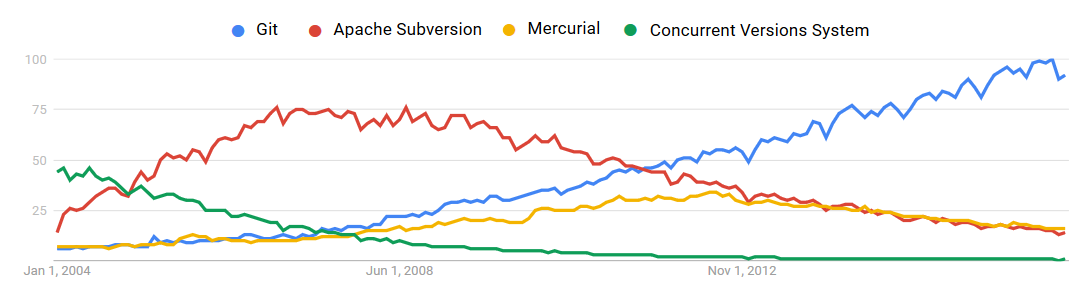
\includegraphics[width=16cm]{vcs_interest}
		\captionsource{Zainteresowanie systemami kontroli wersji w wyszukiwarce Google, dane od stycznia 2004 do stycznia 2017}{\url{https://www.google.com/trends/explore?date=2004-01-01\%202017-01-01\&q=\%2Fm\%2F05vqwg,\%2Fm\%2F012ct9,\%2Fm\%2F08441\_,\%2Fm\%2F09d6g\&hl=en-US}}
		\label{fig:vcs_interest}
	\end{figure}

	Na rysunku~\ref{fig:vcs_interest} przedstawiony jest wykres ilustrujący relatywną popularność czterech znanych systemów kontroli wersji w~wyszukiwarce Google, na przestrzeni ostatnich 13~lat. Uwzględnione zostały dwa scentralizowane (CVS i~Subversion) oraz dwa rozproszone systemy kontroli wersji (Git i~Mercurial). Wyraźnie widać, że popularność tych pierwszych znacząco spadła względem rozproszonego modelu, który wciąż zyskuje na popularności. Przewaga systemu Git nad pozostałymi nie ulega wątpliwości, jest on aktualnie ponad czterokrotnie częściej wyszukiwany w~Google niż Mercurial czy Subversion, co przekłada się na stale rosnącą liczbę użytkowników.

	Obecnie systemy kontroli wersji są tak popularne, że zdecydowana większość programistów korzysta z~nich na~co~dzień. Praca polegająca na wytwarzaniu oprogramowania wykonywana jest najczęściej zespołowo, a~do efektywnej współpracy system kontroli wersji jest bezwzględnie potrzebny. Znajomość i~umiejętność sprawnego korzystania z takich systemów jest więc niezbędna programistom, którzy zamierzają pracować w~większych przedsiębiorstwach i~korporacjach.

	\section{System kontroli wersji Git}

	System kontroli wersji Git\cite{progit}\cite{gajda} stworzony został w 2005 roku, przez zespół programistów pracujących wspólnie nad jądrem Linuksa, w~tym przez Linusa Torvaldsa, twórcę wspomnianego systemu operacyjnego. Wykorzystywali oni wcześniej inny darmowy rozproszony system kontroli wersji, który przestał być ogólnodostępny. W~związku z~tym postanowili napisać własny, doskonalszy od~poprzedniego. Z~założenia miał to~być szybki, rozproszony system, wspierający współbieżną pracę nad różnymi aspektami i~dobrze radzący sobie z~ogromnymi projektami, takimi jak jądro Linuksa.

	\subsection{Cechy charakterystyczne}
	Stworzony przez Linusa Torvaldsa system kontroli wersji Git różni się znacząco od wcześniejszych systemów, szczególnie tych scentralizowanych. W odmienny sposób przechowuje nowe wersje plików. W przeciwieństwie do poprzedników zapamiętuje cały stan repozytorium, a~nie jedynie różnicę pomiędzy plikami. Dla zwiększenia efektywności, jeśli plik nie został zmodyfikowany, to nie jest kopiowany tylko przechowywana jest referencja do~jego aktualnej wersji.

	Kolejną istotną różnicą jest możliwość pracy lokalnej, bez ciągłej potrzeby łączenia się z~serwerem, nawet przy pracy nad projektem zespołowym. System Git pozwala wprowadzać zmiany i~zatwierdzać je bez dostępu do sieci. Komunikacja z innymi jednostkami w~celu synchronizacji danych może odbyć się w~dowolnym momencie. Wcześniejsze scentralizowane systemy, takie jak Subversion, nie pozwalały na taki model pracy. Większość operacji wymagała połączenia z~serwerem, co~wpływało na dłuższy czas wykonywania.

	Git przypisuje do zapisanych stanów projektu czterdziestoznakowe skróty SHA-1. Dzięki tym sumom kontrolnym zauważy każdą, nawet najmniejszą zmianę wprowadzoną na kontrolowanym pliku, niezależnie od sposobu przeprowadzenia modyfikacji.

	Jako najważniejszą zaletę systemu Git powszechnie uznaje się efektywny system rozgałęziania i~łączenia gałęzi. W~przeciwieństwie do starszych systemów kontroli wersji, Git umożliwia natychmiastowe utworzenie nowej gałęzi, oraz bardzo szybkie przełączanie się pomiędzy gałęziami. Ta cecha sprawia, że równoległa praca jest o~wiele mniej problematyczna. Znacząco ułatwia to rozwój oprogramowania jednocześnie w~kilku różnych i~niezależnych kierunkach. Tak optymalne operacje na gałęziach są możliwe dzięki potraktowaniu gałęzi jako wskaźnika na rewizję.

	\subsection{Repozytorium}

	Aby w pełni zrozumieć, czym jest Git, należy zacząć od wytłumaczenia kilku pojęć. Przez zwykłe repozytorium systemu Git określa się folder, przechowujący całą dotychczasową historię projektu i wszystkie zapisane wersje śledzonych plików, oraz przestrzeń roboczą (ang. \textit{working directory}), w której znajdują się bieżące pliki. Git wyróżnia także repozytoria surowe (ang. \textit{bare}), służące przede wszystkim do~synchronizacji i~wymiany zmian. Nie posiadają one obszaru roboczego, ponieważ nie są przeznaczone do tego, aby w~nich pracować.

	Repozytorium systemu Git można samodzielnie utworzyć w dowolnym folderze na dysku, lub pobrać poprzez sklonowanie istniejącego. Pierwsza metoda może dotyczyć zarówno pustego katalogu jak i~takiego, który już zawiera projekt. Podczas inicjalizacji repozytorium zostanie utworzony osobny podkatalog .git, obejmujący wszystkie pliki potrzebne systemowi Git do działania. Pozostała zawartość folderu, w którym utworzono repozytorium, pozostanie niezmieniona. Drugi sposób polega na sklonowaniu istniejącego repozytorium do wybranego katalogu na dysku. Pobrany zostanie folder .git, wraz z całą zawartością, oraz obszar roboczy ze wszystkimi plikami projektu.

	\subsection{Tworzenie rewizji}
	Za każdym razem, kiedy uznamy, że aktualny stan naszego projektu wart jest zapisania, trzeba samodzielnie zatwierdzić wprowadzone zmiany. Odbywa się to dwuetapowo.

	Najpierw należy określić, które pliki powinny zostać zapisane w repozytorium, poprzez zaindeksowanie ich, czyli dodanie do indeksu (ang. \textit{index}, \textit{staging area}) komendą \textit{git add}. Plik index przechowuje listę plików, których zmiany zostaną uwzględnione w~najbliższej rewizji. Mieści się w~podkatalogu .git, stanowiącym integralną część każdego projektu kontrolowanego przez system Git i zawierającym całą dostępną historię, wraz ze~wszystkimi danymi dotyczącymi repozytorium.

	Następnie zatwierdza się zmiany poleceniem \textit{git commit}, w~rezultacie czego powstaje nowa rewizja (ang. \textit{commit}), zawierająca zapisany obraz całego projektu, nazywany czasem migawką (ang. \textit{snapshot}). Wszystkie rewizje przechowywane są w repozytorium i~oznaczone są jednoznacznie je identyfikującą sumą kontrolną. Wyliczona jest przez funkcję skrótu \mbox{SHA-1}, generującą 40-znakowy ciąg na~podstawie zawartości rewizji. Poza zapisanym stanem plików zapamiętywana jest także dokładna godzina zatwierdzenia zmian, autor oraz przodek rewizji (ang \textit{parent commit}). Przodkiem określa się rewizję bezpośrednio poprzedzającą daną rewizję. Warto w tym miejscu zaznaczyć, że rewizje powstałe w~wyniku scalenia gałęzi mają więcej niż jednego rodzica. Więcej na temat gałęzi w~sekcji~\ref{Galezie}.

	Pliki znajdujące się w projekcie kontrolowanym przez system Git można podzielić na następujące kategorie:
	\begin{itemize}
		\item aktualne --- w obszarze roboczym znajduje się identyczna wersja pliku jak w~ostatnio wykonanej rewizji,
		\item zmodyfikowane --- od czasu zatwierdzenia zmian w pliku zostały wprowadzone pewne modyfikacje, niedodane do indeksu (a~więc gdyby w~tym momencie utworzona została rewizja, to nie zawierałaby tych zmian),
		\item zaindeksowane --- od czasu zatwierdzenia zmian plik został zmieniony, a następnie dodany do~indeksu (czyli zarówno w obszarze roboczym, jak i~w~indeksie, znajduje się ta sama wersja --- będzie ona zapisana przy kolejnej rewizji).
		\item nieśledzone - pliki występujące w obszarze roboczym, ale nieznajdujące się ani w~repozytorium, ani w~indeksie --- w~tym stanie jest początkowo każdy nowo dodany do obszaru roboczego plik,
		\item ignorowane --- pliki nieśledzone, wyszczególnione w~specjalnym pliku .gitignore, informującym system Git których plików ma nie uwzględniać i~nigdy nie indeksować.
	\end{itemize}

	\begin{figure}[h]
		\centering
		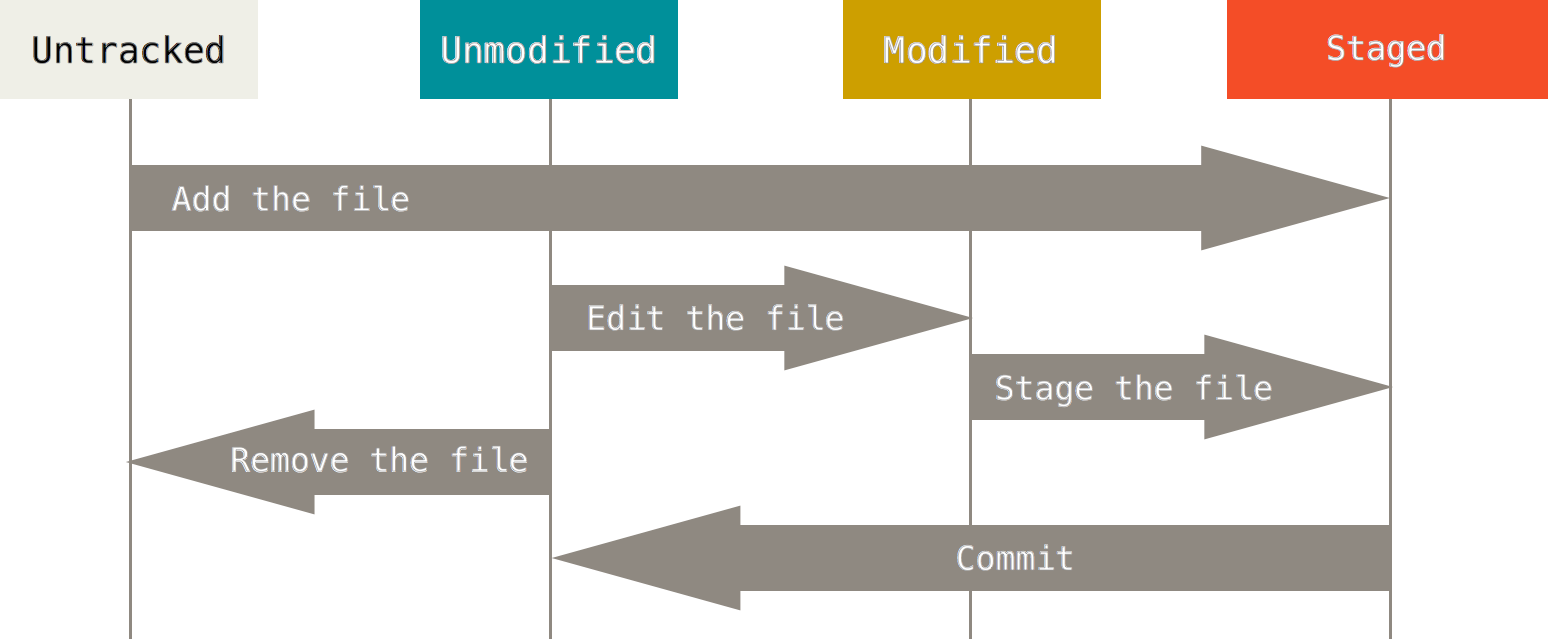
\includegraphics[height=6.5cm]{git_file-types}
		\captionsource{Możliwe stany pliku w systemie Git}{Oryginalna ilustracja angielska : \mbox{\url{https://git-scm.com/book/en/v2/Git-Basics-Recording-Changes-to-the-Repository}}}
		\label{fig:git_file-types}
	\end{figure}
	\FloatBarrier

	\paragraph{Etykiety}
	System Git umożliwia oznaczanie wybranych rewizji etykietami, zwanymi także znacznikami, za pomocą polecenia \textit{git tag}. Etykiety wykorzystywane są najczęściej do oznaczania ważnych wersji projektu, przede wszystkim na gałęzi produkcyjnej przy publikacji nowego wydania. Do wyszukania konkretnej rewizji w~historii projektu konieczne jest podanie skrótu SHA-1, identyfikującego daną rewizję, ale można w~tym celu posłużyć się znacznikiem. Dzięki temu odnalezienie istotnych wersji oprogramowania jest łatwiejsze.

	Etykiety nadawane rewizjom można podzielić na dwa typy:
	\begin{itemize}
		\item lekkie (ang. \textit{lightweight tags}) --- przechowujące jedynie skrót SHA-1 wskazywanej rewizji,
		\item opisane (ang. \textit{annotated tags}) --- zawierające poza skrótem SHA-1 rewizji także datę utworzenia, autora i~opcjonalnie dodatkowy komentarz.
	\end{itemize}

	\subsection{Gałęzie} \label{Galezie} \label{HEAD}
	W systemie Git istotną rolę pełnią gałęzie, będące w rzeczywistości wskaźnikami na rewizje.
	Każde repozytorium zawiera zaraz po utworzeniu dokładnie jedną, domyślną gałąź o nazwie \textit{master}. Wskazuje ona na najnowszą rewizję, czyli na samym początku na rewizję inicjującą. Po wykonaniu operacji zatwierdzenia wskaźnik aktualnej gałęzi automatycznie przesuwa się do przodu, na nowo powstałą rewizję. W~tym miejscu należy przypomnieć, że system Git przyporządkowuje rewizjom skróty \mbox{SHA-1}, służące jako identyfikatory. Dla każdej gałęzi przechowywany jest plik tekstowy, przechowujący skrót rewizji, na którą dana gałąź wskazuje. Oznacza to, że przesunięcie gałęzi sprowadza się jedynie do zmiany identyfikatora \mbox{SHA-1} w~pliku dotyczącym tej gałęzi.

	W systemie Git utworzenie nowej gałęzi jest niemalże natychmiastowe, ponieważ polega jedynie na dodaniu wskaźnika na rewizję. Wiąże się to ze stworzeniem pliku tekstowego, o takiej samej nazwie jak nazwa gałęzi, który zawierać będzie czterdziestoznakowy identyfikator wskazywanej rewizji. Operacja dodawania gałęzi jest bardzo szybka, nie wymaga bowiem kopiowania całego repozytorium.
	Wykonuje się ją poleceniem \textit{git branch}.

	Istnieje także szczególny wskaźnik HEAD, przechowujący informację o aktualnie aktywnej gałęzi. W odróżnieniu od zwykłej gałęzi nie wskazuje on na konkretną rewizję, lecz na gałąź. Jeżeli zostanie utworzona nowa rewizja, to wpis w pliku dotyczącym bieżącej gałęzi uaktualni się. W rezultacie HEAD będzie również wskazywał na najnowszą rewizję, choć zawartość jego pliku nie uległa zmianie~---~wskaźnik HEAD nadal wskazuje na aktywną gałąź.

	\begin{figure}[h]
		\centering
		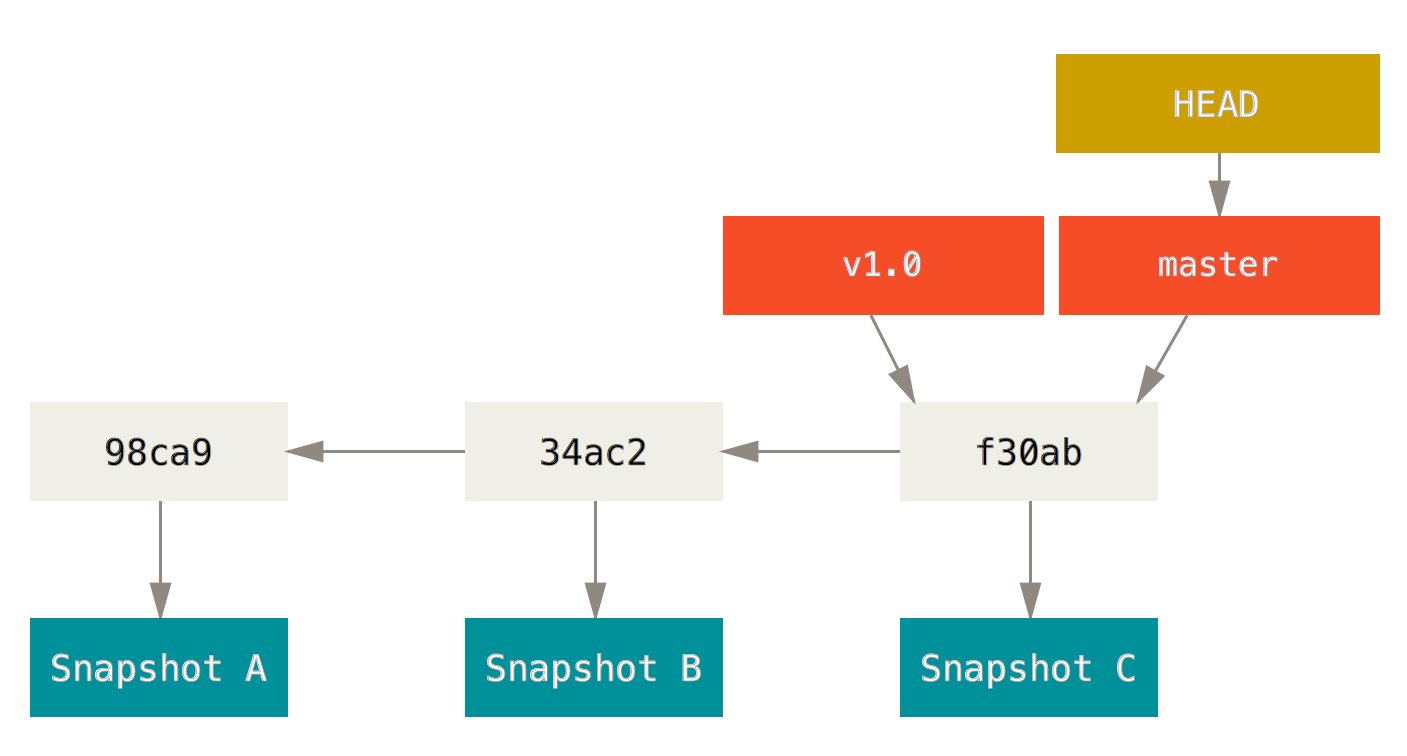
\includegraphics[width=12cm]{git_HEAD}
		\captionsource{Repozytorium zawierające trzy rewizje, z~bieżącą gałęzią \textit{master}}{\url{https://git-scm.com/book/en/v2/Git-Branching-Branches-in-a-Nutshell}}
		\label{fig:git_HEAD}
	\end{figure}

	Na rysunku \ref{fig:git_HEAD} przedstawione jest repozytorium, w którym utworzone zostały trzy rewizje. Ich skróty SHA-1 zaczynają się od następujących ciągów znaków: 98ca9, 34ac2 i f30ab. Każda z nich przechowuje zapamiętany stan projektu, czyli migawkę (ang. \textit{snapshot}). W~prezentowanym repozytorium są dwie gałęzie, \textit{v1.0} oraz \textit{master}. Wskaźnik symboliczny HEAD wskazuje na gałąź \textit{master}, co oznacza, że jest ona gałęzią aktywną.

	System Git umożliwia przełączanie się pomiędzy gałęziami za pomocą polecenia \textit{git checkout}. Przełączenie się na gałąź jest równoznaczne z~przywróceniem obszaru roboczego do stanu, jaki został zapisany we~wskazywanej przez nią rewizji. Możliwe jest również przełączenie się bezpośrednio na konkretną rewizję, niewskazywaną przez żadną gałąź, poprzez podanie jej skrótu SHA-1. Spowoduje to przejście do stanu nazywanego w języku angielskim \textit{detached HEAD}, w~którym żadna gałąź nie jest gałęzią aktywną. Jeżeli w tym stanie wykonana zostanie operacja zatwierdzania, to utworzona rewizja nie będzie zawarta w~żadnej gałęzi, a~co za tym idzie może zostać łatwo utracona. W~związku z~tym nie należy pracować w stanie \textit{detached HEAD}. W~przypadku, w~którym konieczna jest kontynuacja projektu od konkretnej rewizji, należy najpierw utworzyć nową gałąź wskazującą na daną rewizję, a~następnie się na nią przełączyć.

	\subsubsection*{Łączenie gałęzi}
	Zmiany wprowadzone na osobnych gałęziach w systemie Git można połączyć, aby otrzymać wersję projektu zawierającą modyfikacje z kilku gałęzi. Istnieją dwa sposoby na wykonanie operacji łączenia, scalanie (ang. \textit{merge}) oraz zmiana bazy (ang.~\textit{rebase}). Ostateczny rezultat jest identyczny, różnica między tymi sposobami polega przede wszystkim na innej historii projektu.

	\paragraph{Scalanie}

	Łączenie gałęzi poprzez scalanie wykonywane jest poleceniem \textit{git merge}. Integrowanie zmian może być realizowane na gałęziach rozłącznych lub takich, z~których jedna jest zawarta w~drugiej. Przez zawieranie się gałęzi określa się sytuację, w~której jedna gałąź zawiera ciąg rewizji, a~druga składa się z~identycznego ciągu do~którego dodane zostały nowe rewizje. Innymi słowy, z~pierwszej gałęzi można w~prostej linii dotrzeć do drugiej, podążając wzdłuż historii projektu.

	Wykonanie operacji scalania na gałęzi zawartej w dołączanej do niej gałęzi odbywa się poprzez przewinięcie do przodu (ang. \textit{fast forward}). Wskaźnik zawartej gałęzi jest przesuwany do najnowszej rewizji, wskazywanej przez gałąź dołączaną. Ilustracja~\ref{fig:git-merge_ff} przedstawia scalenie gałęzi \textit{master} z~zawierającą ją gałęzią \textit{iss53}, które przewinęło wskaźnik gałęzi \textit{master} do przodu, nie tworząc przy tym nowej rewizji.

	\begin{figure}[h]
		\centering
		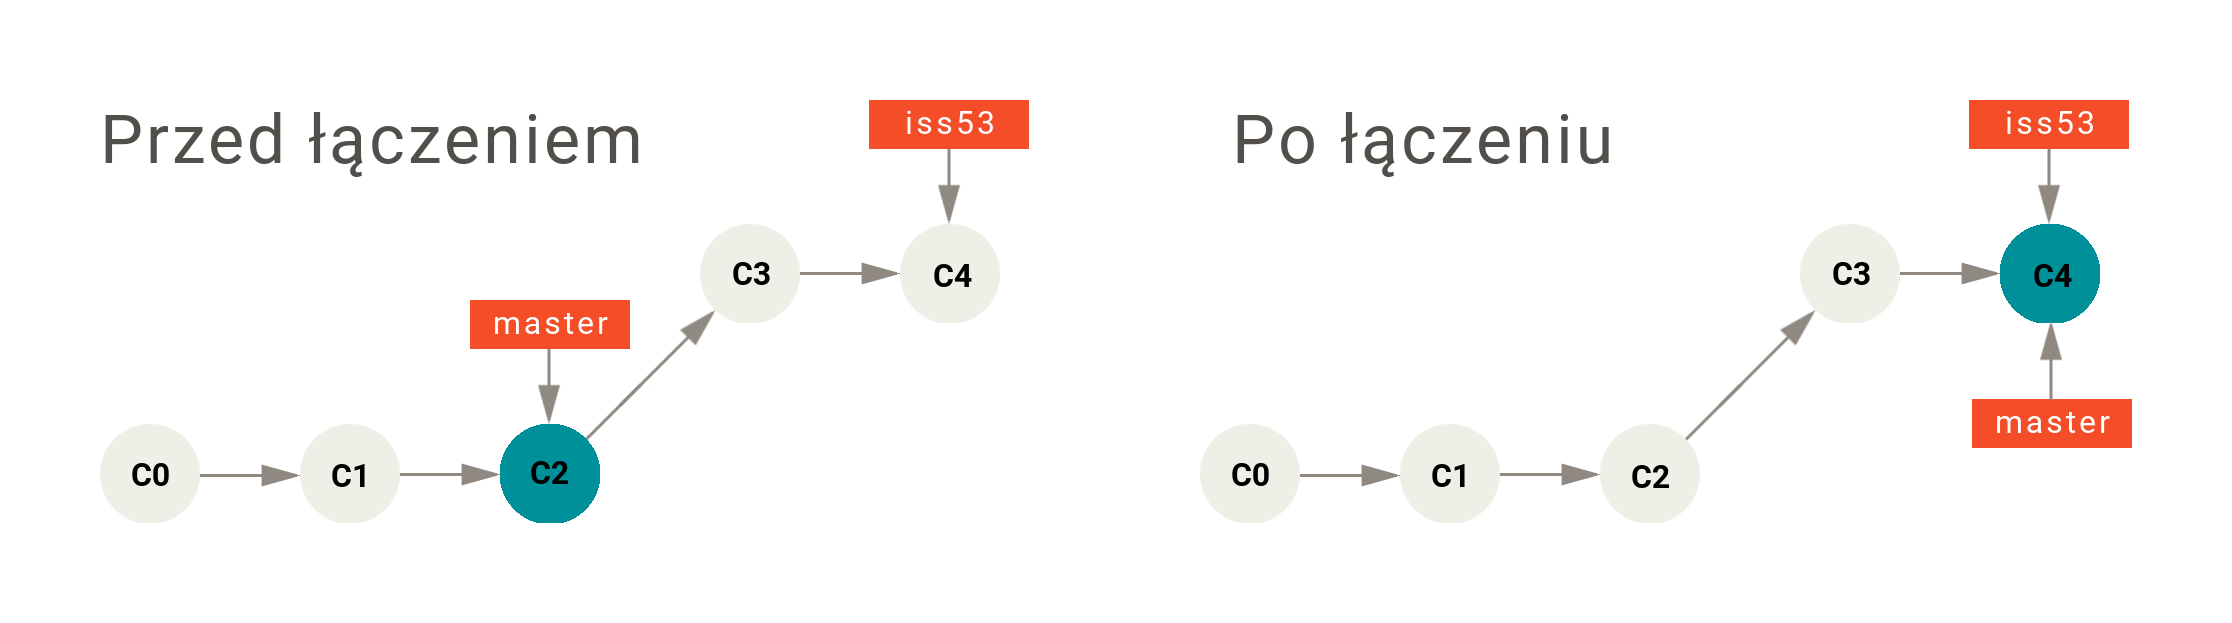
\includegraphics[width=14cm]{git-merge_ff}
		\caption{Działanie operacji scalania poprzez przewinięcie do przodu}
		\label{fig:git-merge_ff}
	\end{figure}

	W przypadku łączenia gałęzi rozłącznych, czyli takich, że~żadna nie jest zawarta w~drugiej, nie jest możliwe scalenie poprzez przewinięcie do~przodu. System Git ustala wówczas wspólnego przodka, czyli rewizję, od~której historie gałęzi różnią się między sobą, oraz rewizje wskazywane przez wskaźniki łączonych gałęzi. Na~podstawie tych trzech migawek wykonywane jest scalenie trójstronne (ang.~\textit{three-way merge}), w~wyniku którego powstaje nowa rewizja. Jest ona szczególna, ponieważ posiada więcej niż jednego przodka.

	\begin{figure}[h]
		\centering
		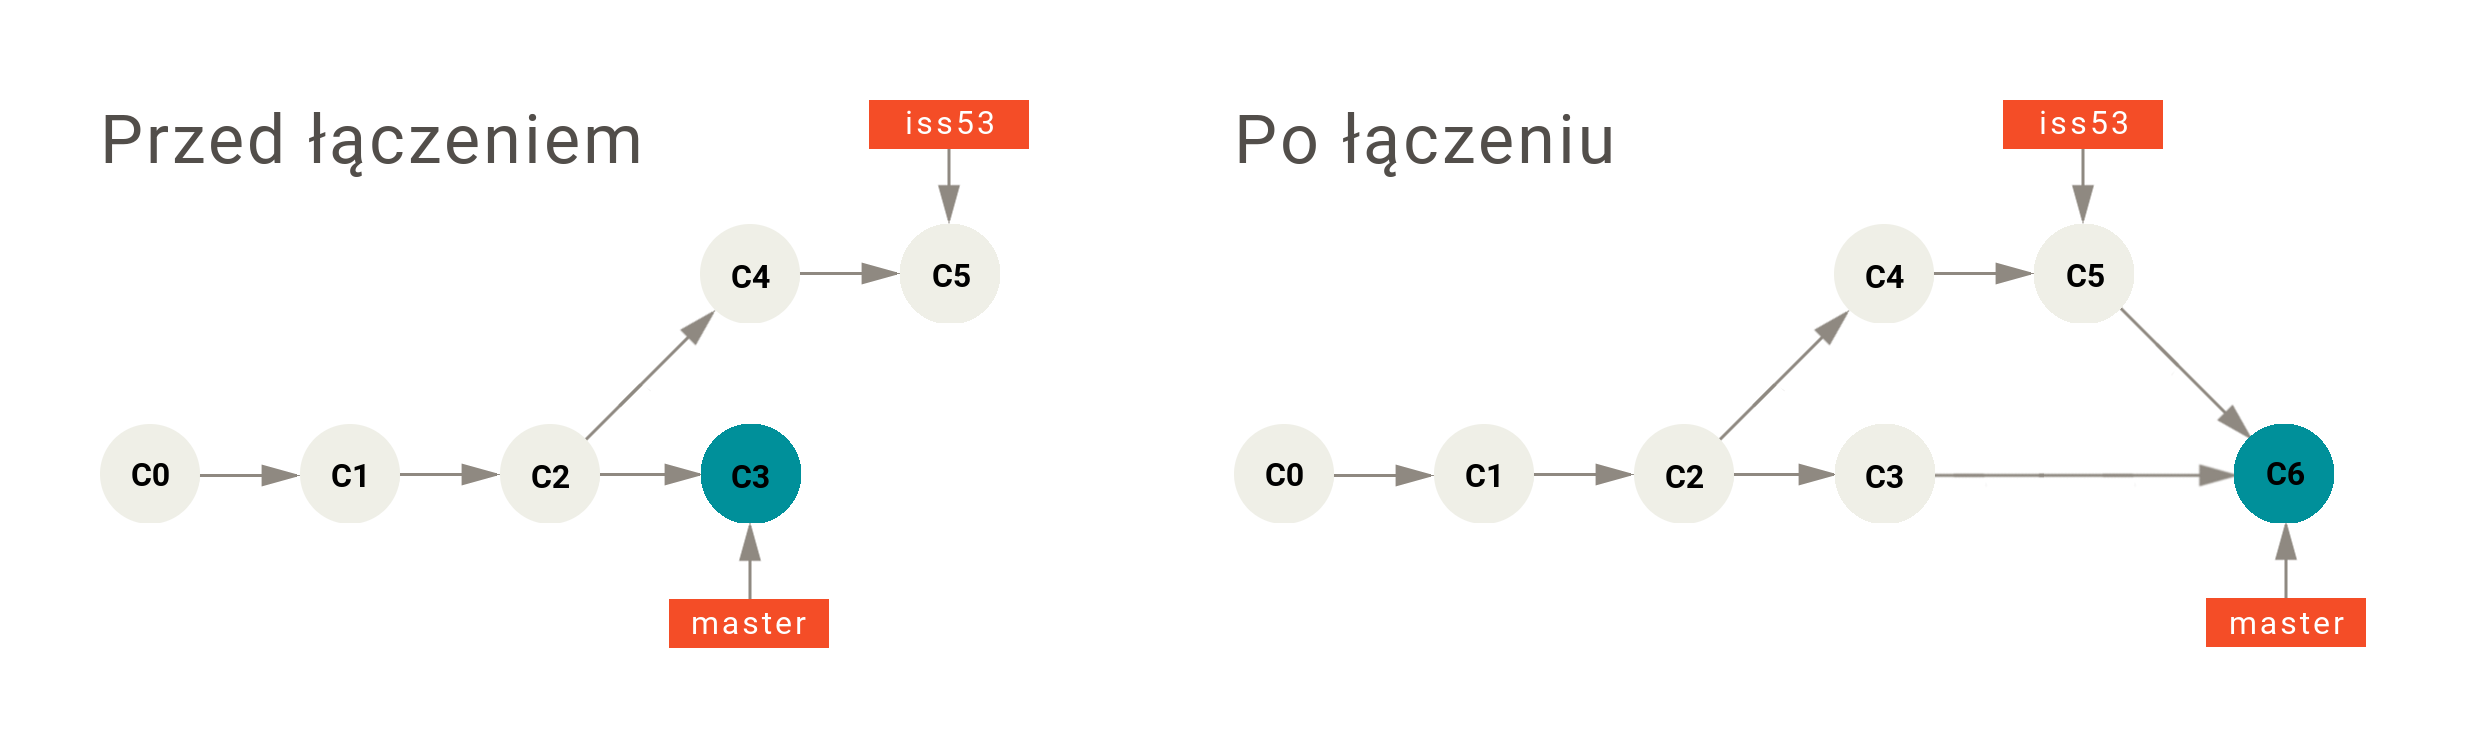
\includegraphics[width=15cm]{git-merge_no_ff}
		\caption{Działanie operacji scalania rozłącznych gałęzi}
		\label{fig:git-merge_no_ff}
	\end{figure}

	Przykład przeprowadzenia operacji scalania rozłącznych gałęzi jest przedstawiony na rysunku~\ref{fig:git-merge_no_ff}. Do gałęzi \textit{master}, która wcześniej wskazywała na rewizję C4, dołączone zostały zmiany z gałęzi \textit{iss53}. W wyniku tego powstała nowa rewizja C5.

	\FloatBarrier

	\paragraph{Zmiana bazy}

	Innym sposobem integracji zmian z różnych gałęzi jest zmiana bazy, wykonywana poleceniem \textit{git rebase}. System Git wyszukuje wspólnego przodka gałęzi i~sprawdza, jakie zmiany zostały przeprowadzone na gałęzi, która ma zostać dołączona. Następnie zmiany te są nakładane na gałąź bazową. W rezultacie utworzone zostają nowe rewizje, a~gałąź bazowa jest zawarta w gałęzi, której baza została zmieniona. Można je teraz scalić poprzez przewinięcie do~przodu. Ostatecznie stan plików projektu jest identyczny z~tym, jaki powstałby w~wyniku operacji scalenia rozłącznych gałęzi. Jedyna różnica jest widoczna w~historii projektu~---~po zmianie bazy jest ona liniowa, a~w wyniku scalenia zawierałaby rozgałęzienia. Przykład działania operacji zmiany bazy przedstawiony jest na rysunku~\ref{fig:git-rebase}.

	\begin{figure}[h]
		\centering
		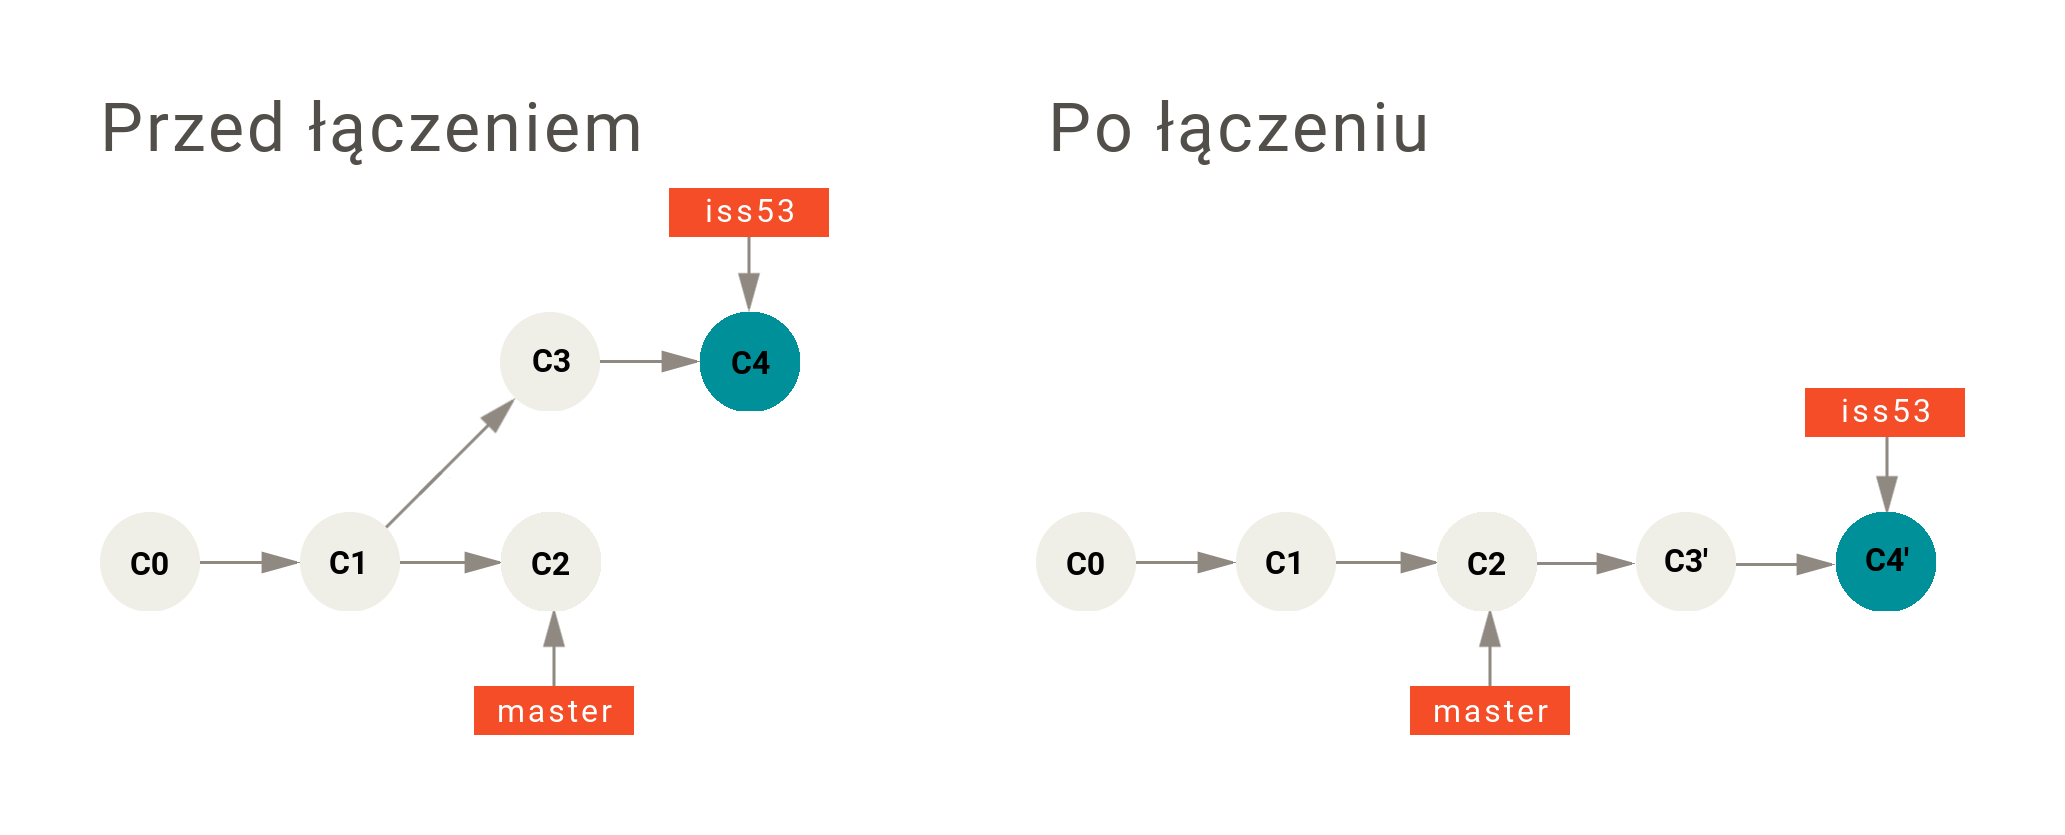
\includegraphics[width=13cm]{git-rebase}
		\caption{Działanie operacji zmiany bazy gałęzi \textit{iss53} }
		\label{fig:git-rebase}
	\end{figure}
	\FloatBarrier

	\subsection{Wycofywanie zmian}
	Jeżeli zajdzie potrzeba wycofania zaindeksowanych zmian lub usunięcia utworzonych rewizji, należy użyć komendy \textit{git reset} systemu Git, wywoływanej w~jednym z~trzech trybów:
	\begin{itemize}
		\item \textbf{\textit{soft}}~---~ aktywna gałąź (wskazywana przez HEAD) przesuwana jest do podanej jako parametr rewizji, a indeks i obszar roboczy pozostają bez zmian,
		\item \textbf{\textit{mixed}}~---~tryb domyślny, w którym aktywna gałąź przesuwana jest do podanej rewizji i dodatkowo zmieniany jest indeks (przywracany do stanu takiego jak w danej rewizji), a obszar roboczy pozostaje bez zmian,
		\item \textbf{\textit{hard}}~---~przesuwana jest aktywna gałąź, a zarówno indeks jak i~obszar roboczy są przywracane do stanu zapamiętanego w podanej rewizji (ten tryb może spowodować nieodwracalną utratę zmian, nawet tych zatwierdzonych).
	\end{itemize}
	Reasumując, polecenie \textit{git reset} z~opcją \textit{hard} wykonuje trzy kroki~---~cofa wskaźnik aktywnej gałęzi, zmienia indeks, a~następnie przywraca stan obszaru roboczego do~stanu zapisanego we wskazanej rewizji. W trybie \textit{mixed} pomijany jest ostatni krok, modyfikujący pliki w~katalogu roboczym. Z~kolei tryb \textit{soft} wykonuje tylko krok pierwszy.

	Komendę \textit{git reset} w trybie \textit{mixed} można wykorzystać do~wykluczenia zaindeksowanego pliku z~indeksu, a~z~opcją \textit{hard} do~usunięcia najnowszych rewizji. Za~pomocą tego polecenia wycofuje się także operację scalania, która utworzyła nową rewizję (nie dotyczy to scalania poprzez przewinięcie do~przodu).

	\subsection{Repozytoria zdalne}
	Do tej pory omówione pojęcia dotyczyły lokalnego repozytorium. System Git umożliwia pracę zespołową, do której niezbędne są zdalne repozytoria, udostępnione w~sieci. Służą one do~synchronizacji zmian w~projekcie, najczęściej wykonanych przez różne osoby. Korzystanie z~repozytorium zdalnego polega przede wszystkim na~pobieraniu i~przesyłaniu do~niego danych, dotyczących wersji projektu i~stanu plików.

	Jeżeli repozytorium lokalne powstało w wyniku wywołania komendy \textit{git clone}, to~jest kopią repozytorium zdalnego, podanego jako parametr polecenia i istnieje między nimi powiązanie.
	Z~jednym repozytorium lokalnym może być związanych kilka różnych repozytoriów zdalnych, które są najczęściej repozytoriami surowymi, czyli nieposiadającymi obszaru roboczego. Powiązanie dodaje się komendą {\textit{git~remote~add}, w~której określa się adres repozytorium zdalnego i~nadaje się mu dowolną nazwę. Domyślnie repozytorium zdalne, które zostało sklonowane, nosi nazwę \mbox{\textit{origin}}.

	\paragraph{Pobieranie zmian}
	Synchronizacja repozytorium lokalnego z~repozytorium zdalnym wymaga pobrania danych z~serwera. Służy do tego polecenie \textit{git fetch}, które pobiera rewizje znajdujące się w repozytorium zdalnym, niewystępujące w~lokalnej historii projektu. Wywołanie tej komendy nie modyfikuje aktualnych plików w~obszarze roboczym, ponieważ zmiany z~serwera zostają pobrane, ale nie zintegrowane z~bieżącą wersją.

	Repozytoria zdalne, tak jak zwykłe repozytoria lokalne, posiadają gałęzie (co~najmniej jedną, domyślnie nazwaną \textit{master}). Pobieranie zmian polega na pobraniu rewizji z konkretnej, zdalnej gałęzi. W celu dołączenia ich do własnej wersji projektu należy połączyć gałęzie~---~zdalną oraz lokalną. Operacja integrowania zmian przebiega w identyczny sposób, jak w~przypadku łączenia dwóch gałęzi lokalnych i~może być przeprowadzona poprzez scalanie lub zmianę bazy.

	Do pobrania zmian z repozytorium zdalnego można zamiast polecenia \textit{git fetch} użyć komendy \textit{git pull}, która najpierw pobiera brakujące rewizje, a~następnie dołącza je do aktywnej gałęzi. Domyślnie operacja łączenia wykonywana jest poprzez scalanie, ale za pomocą odpowiedniego przełącznika można poinformować system Git, aby zamiast tego przeprowadził zmianę bazy.

	\paragraph{Wypychanie zmian}
	Przesyłanie rewizji utworzonych w lokalnym repozytorium na serwer realizowane jest poleceniem \textit{git push}, przyjmującym jako parametry nazwę zdalnego repozytorium oraz zdalną gałąź. Komenda zadziała tylko jeżeli na serwerze nie ma żadnych nowych, niepobranych wcześniej zmian. W~przypadku, w~którym w~repozytorium zdalnym znajdują się rewizje niedołączone do repozytorium lokalnego, próba wypchnięcia własnych zmian zostanie odrzucona. Konieczne będzie pobranie brakujących rewizji i~dołączenie ich do posiadanej wersji projektu. Przesłanie zmian do~repozytorium zdalnego jest możliwe dopiero gdy gałąź zdalna zawiera się w~lokalnej gałęzi.

	\paragraph{Gałęzie śledzące}
	Podczas wykonywania poleceń służących do pobierania lub wypychania rewizji konieczne jest określenie repozytorium zdalnego i~jego gałęzi, z~którą należy zsynchronizować zmiany. System Git umożliwia skonfigurowanie gałęzi lokalnej jako gałęzi śledzącej, mającej bezpośrednie powiązanie ze wskazaną gałęzią z repozytorium zdalnego. Dzięki temu, podczas wykonywania polecenia \textit{git pull} lub \textit{git push} z~gałęzi śledzącej, nie trzeba podawać żadnych parametrów, ponieważ synchronizacja domyślnie przeprowadzana jest z~gałęzią śledzoną.

	Lokalną gałąź śledzącą nazywa się w języku angielskim \textit{tracking branch}, a powiązaną z nią gałąź \textit{upstream branch}. W systemie Git istnieje też termin \textit{remote-tracking branch}, odnoszący się do referencji do zdalnej gałęzi. Wskazuje ona na~rewizję, na~jaką wskazywała dana zdalna gałąź podczas ostatniej komunikacji z~serwerem. W~przeciwieństwie do~zwykłych gałęzi tych referencji nie można samodzielnie przesunąć. Uaktualniają się automatycznie, na skutek wymiany danych z~repozytorium zdalnym.

	\section{Gitflow}

	Praca z~wykorzystaniem systemu Git może przebiegać w~zgodzie ze ściśle określonym cyklem. Ustalenie reguł, których będą przestrzegać wszyscy programiści pracujący nad danym projektem, może znacząco ułatwić synchronizację pracy i~pomóc w~sprawnym zarządzaniu i~wydawaniu nowych wersji oprogramowania. Jedną z~bardziej popularnych metodyk jest Gitflow\cite{gitflow}, opracowana przez Vincenta Driessena. Określa ona cykl pracy, oparty na korzystaniu z~różnych gałęzi, z~których każda ma dokładnie zdefiniowaną rolę.

	\begin{figure}
		\centering
		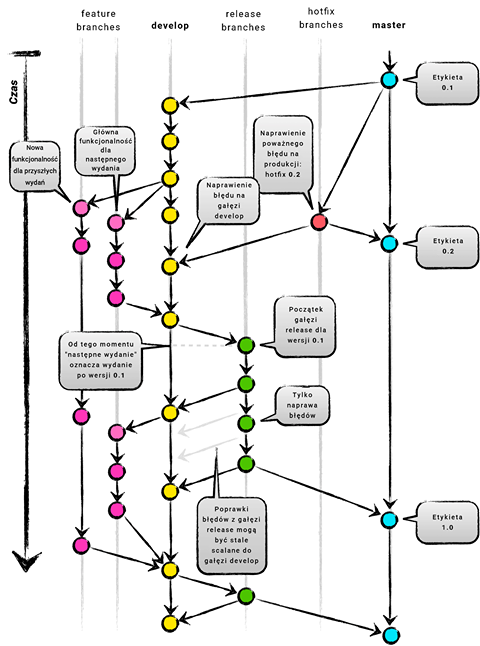
\includegraphics{gitflow}
		\captionsource{Typowy cykl pracy według Gitflow}{Oryginalna ilustracja angielska : \url{http://nvie.com/img/git-model@2x.pngS}}
		\label{fig:gitflow}
	\end{figure}

	\subsection{Podstawowe założenia}

	Zamiast korzystać jedynie z domyślnej gałęzi \textit{master}, Gitflow wykorzystuje dwie główne gałęzie do rejestrowania historii projektu. Jedną z nich jest gałąź produkcyjna \textit{master}, na której przechowywane są tylko oficjalne wydania (ang. \textit{release}). Druga służy jako gałąź deweloperska i jest nazywana \textit{develop}. Przeznaczona jest do integracji bieżących prac programistycznych i nowych funkcji.

	Obie wspomniane gałęzie w idealnym przypadku powinny składać się jedynie z~rewizji powstałych poprzez scalenie gałęzi (ang. \textit{merge commits}). Nie powinno się pracować i~zatwierdzać zmian bezpośrednio na~nich. Wszystkie modyfikacje kodu należy przeprowadzać na osobnych, dedykowanych gałęziach, tworzonych tymczasowo, w~dokładnie określonym celu. Koncepcja Gitflow wyróżnia trzy rodzaje takich gałęzi:
	\begin{itemize}
		\item wprowadzające nowe funkcje (ang. \textit{feature branch}),
		\item przygotowujące do opublikowania nowego wydania (ang. \textit{release branch}),
		\item zawierające niezbędne i szybkie poprawki (ang. \textit{hotfix branch}).
	\end{itemize}
	Z racji braku polskich odpowiedników nazw wymienionych powyżej gałęzi, w przypadku odniesienia do nich, w dalszej części pracy wykorzystywane będzie oryginalne nazewnictwo angielskie.

	Z technicznego punktu widzenia typy gałęzi wykorzystywanych w Gitflow niczym się nie różnią, są to zwykłe gałęzie systemu Git. Są one szczególne jedynie pod względem konkretnych celów, w~jakich są używane i~pewnych ograniczeń dotyczących procesu tworzenia i~łączenia ich. Każdy rodzaj może powstać jedynie przez rozgałęzienie z~określonej gałęzi (produkcyjnej lub deweloperskiej), a~na~koniec musi zostać połączony ze~ściśle ustaloną gałęzią lub gałęziami.

	\subsection{Rozszerzanie funkcjonalności}

	Jednym z podstawowych założeń Gitflow jest implementowanie każdej nowej funkcji oprogramowania na osobnej, dedykowanej gałęzi typu \textit{feature branch}, której nazwa powinna zaczynać się od ,,feature/''. Taka gałąź może powstać jedynie poprzez rozgałęzienie z~głównej gałęzi \textit{develop}. Z założenia ma składać się wyłącznie z rewizji zawierających zmiany dotyczące danej nowej funkcji i~istnieć tak długo, jak długo trwać będzie proces implementacji.

	Kiedy cel zostanie zrealizowany, gałąź typu \textit{feature branch} powinna być połączona z gałęzią \textit{develop}. Istotne jest aby operacja scalania nie została wykonana poprzez przewinięcie do przodu (ang. \textit{fast forward}), czyli zwykłe przesunięcie wskaźnika HEAD. Chodzi o to, by główna gałąź deweloperska nie zawierała wszystkich rewizji pochodzących z gałęzi dołączanej, lecz tylko jedną, powstałą jako łącznik dwóch gałęzi (ang. \textit{merge commit}). W przeciwnym wypadku określenie, które rewizje dotyczą wprowadzenia konkretnej funkcji, wymagałoby dokładnego przejrzenia zawieranych przez nie zmian. A w rezultacie znacznie trudniej byłoby usunąć pojedynczą funkcję z głównej gałęzi.

	Po włączeniu zmian z gałęzi przeznaczonej do implementacji nowej funkcji do głównej gałęzi \textit{develop}, należy usunąć tymczasową gałąź.

	\subsection{Przygotowywanie nowego wydania}

	Kiedy stan kodu aplikacji jest stabilny i działa zgodnie z oczekiwaniami, a wszystkie funkcje które powinny się znaleźć w nowym wydaniu oprogramowania są już zaimplementowane i włączone do głównej gałęzi deweloperskiej, należy rozpocząć proces publikacji nowej wersji. Zgodnie z koncepcją Gitflow, wszystkie niezbędne ostatnie poprawki i drobne zmiany dotyczące przygotowania nowego wydania, powinny zostać przeprowadzone na osobnej, specjalnie utworzonej w tym celu gałęzi, nazywanej \textit{release branch}.

	Tworzenie takiej gałęzi odbywa się poprzez rozgałęzienie z gałęzi \textit{develop}. W~tym momencie ustala się też numer wydania, czyli numer wersji publikowanego oprogramowania. Nazwa gałęzi powinna być formatu ,,release/numer-wydania''.
	Od tego momentu wszystkie zmiany zachodzące na~głównej gałęzi \textit{develop} będą dotyczyć następnej publikacji i~nie zostaną uwzględnione w aktualnym wydaniu. Dzięki utworzeniu gałęzi typu \textit{release} prace mogą iść dwutorowo,  poprzez przygotowywanie publikacji nowej wersji, oraz równolegle rozwijanie i~rozszerzanie funkcjonalności oprogramowania. Przygotowanie do wydania obejmuje korektę drobnych mankamentów, jak literówki i~inne niewielkie niedociągnięcia, a~także naprawę odkrytych podczas testowania błędów.

	W momencie, w którym oprogramowanie będzie już przygotowane do opublikowania, należy scalić gąłąź \textit{release} z~główną gałęzią produkcyjną \textit{master}. Analogicznie jak w~przypadku scalania gałęzi typu \textit{feature branch}, należy  zwrócić uwagę, aby operacja połączenia nie polegała na przewinięciu do przodu. Konieczne jest aby~w~wyniku jej wykonania utworzona została nowa rewizja. Należy jej nadać etykietę (ang. \textit{tag}) z~numerem wydania, aby ułatwić wyszukiwanie konkretnych wersji oprogramowania na gałęzi produkcyjnej. Następnie należy również scalić gałąź dotyczącą najnowszego, opublikowanego właśnie wydania, z~gałęzią \textit{develop}. Gałęzie typu \textit{relese} są tymczasowe, więc po włączeniu jej do obu głównych gałęzi należy ją usunąć.

	\subsection{Naprawa błędów wymagających szybkiego rozwiązania}

	Kolejnym typem gałęzi wykorzystywanych w~koncepcji Gitflow są gałęzie nazywane \textit{hotfix branches}, przeznaczone do~naprawy niecierpiących zwłoki błędów, odkrytych w~opublikowanym oprogramowaniu, najczęściej zgłoszonych przez użytkowników końcowych. Dotyczy to takich wad i~problemów, które są zbyt poważne, aby mogły zostać naprawione dopiero w~następnym wydaniu. W~przypadku mniej istotnych niedociągnięć wystarczy poprawić dane aspekty w~normalnym trybie pracy i~włączyć je do gałęzi \textit{develop}. Zostaną uwzględnione przy kolejnej publikacji przez gałąź typu \textit{release}.

	Gałąź typu \textit{hotfix} jest jedynym rodzajem gałęzi, który powstaje poprzez rozgałęzienie z~głównej gałęzi produkcyjnej \textit{master}. Jej nazwa powinna zaczynać się od~wyrażenia ,,hotfix/''. Taka gałąź zawiera tylko zmiany dotyczące naprawy wykrytego błędu, które powinny być wykonane w~możliwie najkrótszym czasie. Kiedy problem zostanie rozwiązany, przeznaczoną mu gałąź należy połączyć z~powrotem z~gałęzią \textit{master}. W~tym przypadku również należy dokonać łączenia nie poprzez przewijanie do przodu. W rezultacie na głównej gałęzi produkcyjnej powstaje nowa rewizja, której należy nadać etykietę z~kolejnym numerem wersji. Skutkiem jest publikacja nowego wydania oprogramowania, która, w~przeciwieństwie do~procesu z~wykorzystaniem gałęzi typu \textit{release}, nie była planowana.

	Kolejnym krokiem jest scalenie gałezi \textit{hotfix} z~główną gałęzią \textit{develop}. Jeżeli istnieje w~danym momencie gałąź typu \textit{release}, to do niej również należy włączyć zmiany dotyczące naprawy błędu. Na koniec należy usunąć tymczasową gałąź.

	\begin{figure}
		\centering
		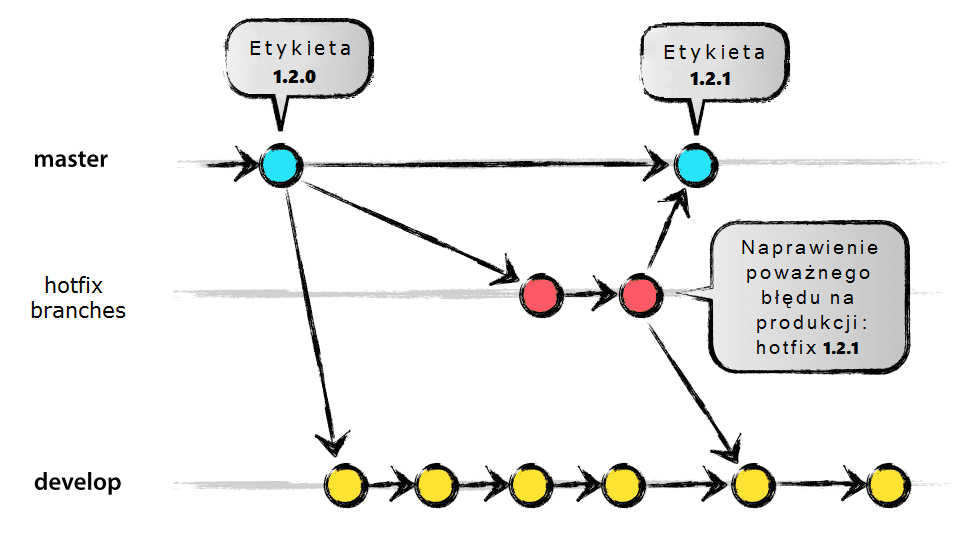
\includegraphics[height=5cm]{gitflow_hotfix}
		\captionsource{Wykorzystanie gałęzi typu \textit{hotfix}}{Oryginalna ilustracja angielska : \url{http://nvie.com/img/hotfix-branches@2x.png}}
		\label{fig:gitflow_hotfix}
	\end{figure}

	\chapter{Projekt} \label{Projekt}

	\section{Założenia}
		
	Głównym celem samouczka GITar-Hero jest zapoznanie użytkownika z~podstawowymi poleceniami systemu kontroli wersji Git, w~sposób przyjemny i~zrozumiały. Gra, przez połączenie nauki i~rozrywki, ma za zadanie zachęcić i~ułatwić proces uczenia się. Kolorowa i~ruchoma grafika 3D uatrakcyjnia tę naukę, a~możliwość zdobywania punktów i~naturalna chęć osiągnięcia jak najlepszego wyniku dodatkowo mobilizuje użytkownika.

	Z~założenia, ważniejsze od dogłębnego zrozumienia strony teoretycznej systemu Git, było nauczenie właściwego korzystania z~poleceń. Gra ma służyć jako samouczek, uczący praktycznego wykorzystania systemu wersji i~pokazujący typowy scenariusz, jaki najczęściej występuje podczas wytwarzania oprogramowania. Po~zagraniu w~grę użytkownik powinien już swobodnie wykonywać komendy systemu Git, zarówno pracując indywidualnie, jak i~podczas współpracy z~zespołem. 
	
	Celem było pokazanie, że~wbrew panującej powszechnie opinii, korzystanie z systemu kontroli wersji Git nie musi przysparzać problemów ani trudności. Ponadto gra ma przyzwyczaić użytkownika do korzystania z~wiersza poleceń. Opanowanie komend, jakie należy wprowadzać w~konsoli, z~reguły daje możliwość używania dowolnego programu z~graficznym interfejsem do obsługi systemu Git. W~drugą stronę taka zależność nie występuje. W~związku z~tym, tylko umiejętność korzystania z~systemu Git w~wierszu poleceń pozwala swobodnie korzystać z~tego systemu kontroli wersji, niezależnie od środowiska i~zainstalowanych programów.
	 
	\section{Przebieg gry}
	
	Gra zaczyna się od krótkiego wprowadzenia, informującego użytkownika, na czym będzie polegała rozgrywka i~do czego służą poszczególne elementy interfejsu. Po~zapoznaniu się z~krótką instrukcją rozpoczyna się gra. U~góry, po prawej stronie, wyświetla się aktualne zadanie i~pierwszy krok, który należy wykonać. Głównym odbiorcą aplikacji jest osoba początkująca, nieznająca poleceń systemu Git. Z tego względu pojawia się podpowiedź sygnalizująca,
	że można otworzyć zakładkę pomocy aby dowiedzieć się czym jest repozytorium sytemu kontroli wersji i~jak je zainicjować. 
	Pomoc zawiera wszystko, co gracz musi wiedzieć, aby poprawnie wykonać dany krok. Po wprowadzeniu przez niego właściwego polecenia i~zatwierdzeniu go poprzez przycisk Enter, aktualny krok zostaje zaliczony i~następuje przejście do kolejnego. Dodatkowo w~katalogu projektu, po lewej stronie, pojawiają się aktualne pliki, jakie znajdują się w~folderze z~repozytorium. Poza tym akcje wykonywane na repozytorium są odwzorowywane przez grafikę 3D, która reaguje odpowiednio na wpisane komendy. Obrazuje to, jak wywołane polecenie wpływa na~stan repozytorium i~pozwala użytkownikowi lepiej zrozumieć skutki wykonywanych komend.

	Po wykonaniu przez użytkownika wszystkich kroków zadania, otrzymuje on punkty. Ich liczba jest zależna od czasu, jaki pozostał do końca zadania. Im szybciej gracz ukończy, tym więcej punktów dostanie. Możliwe jest także nieotrzymanie żadnej nagrody za wykonanie zadania, jeżeli przekroczony zostanie przydzielony do niego czas. Dodatkowo każda błędnie wprowadzona komenda skutkuje zmniejszeniem liczby posiadanych przez użytkownika punktów.
	
	Kolejne zadania, jakie musi wykonywać gracz, są zależne od jego umiejętności. Przechowywane są statystyki dotyczące wprowadzonych komend i~liczby popełnionych błędów. Jeżeli w krokach dotyczących określonego polecenia użytkownik często się mylił, to promowane będą zadania zawierające tę komendę. Nowe zagadnienia będą wdrażane dopiero, gdy wskaźnik znajomości polecenia będzie odpowiednio wysoki. Jest on wyliczany na podstawie liczby prób i~błędów, przy czym ostatnie próby mają większą wagę.
	
	Poziom trudności zadań stopniowo rośnie, zawierają one coraz więcej kroków. Jeżeli użytkownik nie będzie potrafił wykonać aktualnego kroku, może w~dowolnej chwili wpisać w~konsoli 'help'. Otworzy się wówczas pomoc i~gracz będzie mógł odnaleźć potrzebne mu informacje.

	Po przejściu całego scenariusza wyświetli się podsumowanie, zawierające liczbę zdobytych przez gracza punktów oraz podstawowe statystyki, takie jak informacja o~popełnionych błędach i~komendach, z~którymi miał najwięcej problemów. Ukończenie rozgrywki w krótkim czasie skutkuje przyznaniem użytkownikowi dodatkowej nagrody, w~postaci bonusowych punktów.
	
	\section{Zadania}
	
	Scenariusz rozgrywki składa się z~zadań zawierających niezbędne komendy do typowego wykorzystania systemu kontroli wersji Git. Pierwszym terminem, z~jakim zapoznaje się użytkownik, jest repozytorium. Przedstawiane są dwie podstawowe metody pozyskania go~---~poprzez sklonowanie istniejącego lub przez założenie nowego w~wybranym folderze z~projektem. W~kolejnym etapie wprowadzane są pojęcia takie jak przestrzeń robocza, indeks, indeksowanie plików, zatwierdzanie zmian i~rewizja. Gracz uczy się rozróżniać pliki aktualne, zmodyfikowane, zaindeksowane lub nieśledzone. Przed wprowadzeniem kolejnych poleceń i~terminów zadania koncentrują się na tej tematyce, aby użytkownik zdążył je dobrze opanować. 
	
	Po wykonaniu kilku zadań dotyczących wspomnianych wyżej zagadnień, użytkownik uczy się o~gałęziach, poznaje sposoby tworzenia ich i~przełączania się między nimi. Wprowadzane są też pojęcia takie jak gałąź tematyczna, poświęcona konkretnej dodatkowej funkcji aplikacji (ang. \textit{feature branch}). Przy okazji nadal utrwalane są komendy przedstawione w pierwszych zadaniach, dotyczące indeksowania plików i~zatwierdzania zmian. 

	Kolejnym etapem jest nauka łączenia gałęzi. Rozróżnione są przy tym odmienne sposoby na wykonanie tej operacji, takie jak scalanie i zmiana bazy. Następnie pojawia się podstawowy sposób wycofywania zmian i~usuwania wykonanych wcześniej rewizji.

	Kiedy użytkownik opanuje już komendy i~sposób pracy w~lokalnym repozytorium, zapoznaje się z~pojęciem zdalnego repozytorium oraz sposobami komunikacji i~synchronizacji z~nim. W~zadaniach pojawiają się komendy dotyczące ściągania i~przesyłania zmian. Poruszany jest także temat zdalnych gałęzi i~sposoby skonfigurowania lokalnej gałęzi śledzącej zdalną.
	
	Podczas nauki poleceń systemu Git użytkownik zapoznaje się też z~dobrymi praktykami i~metodyką Gitflow, co uczy go właściwych nawyków i~odpowiedniego porządkowania pracy nad projektem. Zaznajamia się z~koncepcją tworzenia osobnych gałęzi, przeznaczonych do implementacji nowych funkcji lub naprawy błędów.
	
	Zadania są podzielone na kroki, dzięki czemu gracz uczy się charakterystycznych sekwencji poleceń, które często występują w rzeczywistych sytuacjach. Ma to również na celu zautomatyzowanie zachowania użytkownika w~prawdziwych przypadkach, z~którymi może się spotkać w~domu lub pracy. W~systemie Git możliwe jest czasem użycie kilku różnych poleceń, aby osiągnąć ten sam rezultat. Zadania i~kroki dopuszczają wszystkie właściwe komendy.
	
	\subsection{Pomoc}
	
	Wszystkie materiały dydaktyczne znajdują się w~pomocy, podzielonej na zakładki, z~których każda dotyczy jednej komendy lub terminu. Jej treść wystarcza, aby osoba nieznająca poleceń systemu Git była w~stanie poprawnie wykonać zadania ze scenariusza rozgrywki. W~przypadku niektórych pojęć jest jednak bardziej obszerna i~wykracza poza wymaganą do przejścia gry wiedzę. Zawiera informacje, które uznano za szczególnie istotne i~przydatne do właściwego zrozumienia systemu Git.
	
	Za każdym razem, gdy podczas rozgrywki w jednym z kroków zadania pojawia się nowe polecenie, pomoc otwiera się automatycznie na odpowiedniej zakładce. Użytkownik może poświęcić dowolnie dużo czasu na zaznajomienie się z~jej treścią, a~ponadto w każdej chwili ma możliwość ponownego przeczytania informacji dotyczących wcześniejszych poleceń.  
	
	\subsection{Punkty za rozwiązanie}

	W projekcie wprowadzono elementy gamifikacji, takie jak punkty za rozwiązanie zadań. Mają one za zadanie zwiększyć zaangażowanie użytkownika. Z~każdym rozegraniem, gracz będzie starać się poprawić swój dotychczasowy wynik. W ten sposób co raz szybciej i~pewniej będzie korzystał z~poleceń systemu Git. Ponadto punkty wprowadzają element rywalizacji pomiędzy użytkownikami, którzy będą dążyć do osiągnięcia jak najlepszego wyniku.

	Punkty możliwe do otrzymania za zadanie obliczane są na podstawie liczby kroków~---~im bardziej złożone zadanie, tym wyżej punktowane. Ostateczna nagroda, jaka przyznawana jest graczowi za~wykonanie zadania, wyliczana jest jako procent maksymalnej liczby punktów, zależny od~czasu rozwiązywania. Dzięki temu użytkownik, który potrafi szybko wykonywać kolejne kroki, osiągnie lepszy wynik. Żeby zapobiec sytuacji, w~której prędkość stałaby się bardziej istotna niż dokładność, za~błędnie wprowadzone komendy gracz karany jest odjęciem określonej liczby punktów.
	
	\chapter{Implementacja} \label{Implementacja}

	\section{Wykorzystane technologie}

	\subsection{JavaScript}

	\textit{JavaScript}\cite{js} jest wysokopoziomowym, skryptowym, wieloparadygmatowym, słabo typowanym językiem programowania. Swoją popularność zawdzięcza szerokiemu zastosowaniu w implementacji aplikacji internetowych. Jest wpierany głównie przez przeglądarki internetowe, może być jednak wykonywany również po stronie serwera, np. w środowisku uruchomieniowym \textit{node.js}.

	\textit{JavaScript} jest językiem zorientowanym prototypowo. Nie istnieje w nim pojęcie klasy, choć w najnowszym standardzie języka została ona dodana do składni (jest to jednak tzw. lukier składniowy). Ponowne wykorzystanie zdefiniowanych zachowań, znane z klas w obiektowych językach programowania, realizowane jest przez dekorację istniejących obiektów, które stanowią później prototypy.

	Funkcje w języku \textit{JavaScript} są typem pierwszoklasowym. Oznacza to, że mogą one być przypisywane do zmiennych, czy dodawane do tablic. Można również konstruować funkcje wyższego rzędu, czyli takie, które przyjmują jako argument funkcję, lub zwracają funkcję.

	\subsection{Redux} \label{Redux}

	Wymagania dotyczące aplikacji przeglądarkowych stały się na tyle skomplikowane, że interfejs użytkownika jest bardzo złożony i może składać się z wielu elementów. Zarządzanie stanem takich aplikacji jest trudne, ponieważ występuje wiele zależności między komponentami. Może to doprowadzić do sytuacji, w której nie jest jasne co tak naprawdę się dzieje, a znalezienie błędów czy rozszerzenie funkcjonalności staje się zadaniem bardzo czasochłonnym.

	Jedną z bibliotek pomagających w rozwiązaniu tego problemu jest \textit{Redux}\cite{redux}. Jej głównym założeniem jest przejrzysty stan aplikacji, który może się zmieniać tylko w określonych momentach i~zawsze w~przewidywalny sposób.

	Stan w \textit{Reduxie} zdefiniowany jest jako zwykły obiekt o~strukturze drzewa, zawierający wszystkie możliwe informacje, jakie są potrzebne aby jednoznacznie określić i móc odtworzyć identyczną sytuację w aplikacji. Nie może on być modyfikowany, jest tylko do odczytu. Jedynym sposobem na jego zmianę jest wyemitowanie akcji, będącej również obiektem zawierającym obowiązkowo pole typ i dowolne inne potrzebne atrybuty. Zadaniem akcji jest przejrzysty opis tego, co się wydarzyło w~aplikacji, dzięki czemu dokładnie wiadomo czy i jak powinien zmienić się stan.

	Kluczowym elementem \textit{Reduxa} są specyficzne funkcje, nazywane w języku angielskim \textit{reducers}, które definiują jak konkretna akcja wpływa na stan. Każda funkcja \textit{reducer} musi spełniać określone wymagania. Jako parametry przyjmuje zawsze tylko i~wyłącznie obecny stan aplikacji i wyemitowaną akcję, a zwraca nowy obiekt stanu, w jakim znajduje się aplikacja na skutek wykonanej akcji. Ważne jest także aby \textit{reducer} był przewidywalny i~deterministyczny. Oznacza to, że określony stan aplikacji i~określona akcja spowodują powstanie zawsze takiego samego stanu. Dodatkowo taka funkcja nie może mieć żadnych skutków ubocznych. W dużych projektach wskazane jest napisanie kilku takich funkcji, z~których każda wpływa tylko na określoną część stanu. Ułatwia to utrzymanie zrozumiałego kodu, który można łatwo rozwijać i~modyfikować.

	Podsumowując, \textit{Redux} opiera się na trzech fundamentalnych zasadach:
	\begin{itemize}
		\item cały stan aplikacji jest opisany przez pojedynczy obiekt o strukturze drzewa,
		\item jedynym sposobem aby zmienić stan aplikacji jest wyemitowanie akcji,
		\item wpływ danej akcji na sposób przekształcenia stanu określają funkcje zwane \textit{reducers}.
	\end{itemize}

	Popularność biblioteki \textit{Redux} zasłużenie rośnie, ze~względu na~prostotę i~korzyści, jakie daje przestrzeganie opisanych wyżej trzech podstawowych reguł. Zdecydowano się skorzystać z~tej biblioteki ponieważ jest łatwa w~użyciu i~pozwala w~wygodny sposób zarządzać stanem aplikacji.

	\subsection{React.js}

	 Jako bibliotekę do budowania interfejsu użytkownika wybrano bibliotekę \textit{React}\cite{react}.
	 Została ona stworzona w 2013 roku przez zespół programistów Facebooka, aby rozwiązać problem tworzenia dynamicznych aplikacji internetowych, w których nieustannie zmienia się to, co należy wyświetlać. Początkowo nie była ona ogólnodostępna, ale aktualnie jest rozpowszechniana na zasadzie otwartego oprogramowania (ang. \textit{open-source}).

   \textit{React} opiera się na koncepcji niezależnych komponentów, nadających się do~wielokrotnego wykorzystania, z~których można komponować skomplikowane widoki. Są to obiekty JavaScript, reprezentujące fragmenty interfejsu użytkownika, mające określoną strukturę i~funkcjonalność. Każdy komponent musi implementować metodę \textit{render()}, odpowiedzialną za wyświetlenie komponentu w przeglądarce. W wartości zwracanej przez tę metodę mogą pojawić się zarówno znaczniki HTML jak i instancje zdefiniowanych wcześniej komponentów. Aplikacje internetowe korzystające z biblioteki \textit{React} budowane są zwykle na zasadzie drzewa komponentów. Tworzony jest jeden komponent nadrzędny, w którym zagnieżdżone są kolejne. Wzorzec ten pozwala zachować modułowość aplikacji.

   Komponenty czerpią wiedzę na temat wyświetlanych informacji z dwóch źródeł - właściwości (\textit{props}) oraz stanu (\textit{state}). Właściwości są obiektem reprezentującym parametry wejściowe podane podczas wywołania komponentu w komponencie nadrzędnym, natomiast stan jest obiektem widocznym i modyfikowalnym tylko wewnątrz danego komponentu. Zmiana stanu komponentu powoduje wywołanie jego metody \textit{render()} i, co za tym idzie, rekursywnego wywoływania metod \textit{render()} komponentów zagnieżdżonych. Efektem tej operacji jest modyfikacja odpowiednich węzłów obiektowego modelu dokumentu (ang. \textit{DOM}) przeglądarki i ostatecznie przerysowanie strony przez przeglądarkę. Należy zaznaczyć, że \textit{React} jest dobrze zoptymalizowany pod kątem renderowania strony. Na szczególną uwagę zasługuje mechanizm wirtualnego obiektowego modelu dokumentu (ang. \textit{virtual DOM}). Polega on na utrzymywaniu kopii DOM reprezentowanej przez zwykłe obiekty JavaScript. Operacje na tych obiektach są znacznie mniej kosztowne, ponieważ nie zmuszają przeglądarki do ponownego renderowania strony. Właściwy DOM jest modyfikowany jedynie w przypadku stwierdzenia różnic między nim a wirtualnym DOM.

   Istotne ułatwienie dla procesu implementacji komponentów stanowi nakładka JSX. Jest to rozszerzenie składni języka JavaScript pozwalające w wygodny sposób używać tagów HTML oraz wywoływać wcześniej zdefiniowane komponenty w kodzie aplikacji. Używanie JSX jest zalecane przy tworzeniu aplikacji opartych o bibliotekę \textit{React} przez samych jej twórców, ponieważ nie tylko ułatwia proces implementacji, ale również zwiększa czytelność kodu.

   Zdecydowano się na wykorzystanie biblioteki \textit{React.js}, ponieważ dzięki abstrakcji operacji na elementach DOM na operacje na komponentach, pozwala ona przy stosunkowo niewielkim nakładzie pracy tworzyć aplikacje działające szybko i niezawodnie.

	\subsection{Babylon.js}

	\textit{Babylon.js}\cite{babylon} jest otwartą biblioteką \textit{WebGL} napisaną w \textit{TypeScript} i~wykorzystywaną przede wszystkim do tworzenia gier wideo w~przeglądarkach. Pierwsza odsłona została wydana w~2013~roku. Głównymi twórcami są David Cotuhe oraz David Rousset. Jako, że \textit{Babylon.js} jest silnikiem 3D, posiada wiele przydatnych narzędzi do~tworzenia, wyświetlania i~teksturowania szkieletów w~przestrzeni. Przez to, że~kierowana jest głównie do twórców gier, posiada również dodatkowe funkcje takie jak generowanie krawędzi czy tworzenie obiektu na podstawie mapy wysokości. Ponadto zapewnia natywną detekcję kolizji, grawitację sceny oraz wbudowane kamery, takie jak kamera śledząca, automatycznie podążająca za obiektem.

	Jako alternatywa rozważana była biblioteka \textit{Three.js} wydana w 2009 roku, również oparta na~\textit{WebGL}. Po zapoznaniu i~przetestowaniu obu silników wybór padł na \textit{Babylon.js}. Przyczyniły się do tego przede wszystkim prostota użycia oraz płynność, którą zapewniał w przeciwieństwie do \textit{Three.js}. Przy renderowaniu sceny o podobnej zawartości i szczegółowości, \textit{Babylon.js} okazał się wydajniejszy. Poza tym biblioteka ta jest dobrze udokumentowana i~posiada bogatą bazę poradników, a~społeczność wykorzystująca tę bibliotekę jest bardzo liczna i~stale rośnie.

	\section{Scenariusz rozgrywki}

	\subsection{Struktura} \label{Struktura}

	Scenariusz rozgrywki to skierowany graf ważony, którego wierzchołki są~zadaniami, składającymi się~z~kilku kroków. Zdecydowano się na strukturę grafu ze~względu na~to, że~daje ona możliwość sekwencjonowania zadań, a~zarazem pozwala wprowadzić element losowości. Jeżeli z~wierzchołka dotyczącego jakiegoś zadania wychodzi kilka krawędzi, to kolejny węzeł, czyli kolejne zadanie, wybierane jest w~sposób losowy spośród sąsiadów aktualnego wierzchołka. Uwzględniane są przy~tym wagi krawędzi, generowane dynamicznie na podstawie statystyk gracza dotyczących znajomości poszczególnych zagadnień. Im~zadanie zawiera więcej kroków wymagających użycia problematycznych dla użytkownika poleceń, tym większą wagę ma~krawędź prowadząca do~tego węzła. A w rezultacie większe jest prawdopodobieństwo, że~wylosowane zostanie to zadanie.
	
	Dzięki takiej reprezentacji nigdy nie zdarzy się sytuacja, w~której następnym zadaniem będzie zadanie nieadekwatne do aktualnego stanu repozytorium, ale możliwe jest dynamiczne wybieranie zadań, uwzględniające umiejętności gracza.

	\subsubsection{Konstrukcja zadania}
	Pojedyncze zadanie reprezentowane jest w postaci obiektu, który składa się z pól opisanych poniżej.
	\begin{description}
	\item[Identyfikator] \hfill \\
		Unikalny numer zadania, na podstawie którego można dowiedzieć się, ile zadań zostało już wcześniej wykonanych.
		
	\item[Tytuł] \hfill \\
		Krótki tytuł zadania naprowadzający na poruszaną przez nie tematykę.
	
	\item[Opis] \hfill \\
		Opis zadania służy ukazaniu użytkownikowi celu oraz problemu, jaki należy rozwiązać w danym zadaniu. Może to być na przykład rozszerzenie funkcjonalności lub naprawa błędu.
		
	\item[Czas] \hfill \\
		Każde zadanie ma przydzielony czas, przeznaczony na jego wykonanie. Jeżeli gracz ukończy wszystkie kroki danego zadania w czasie krótszym niż ustalony, to otrzyma nagrodę w postaci punktów. Ich liczba zależna jest od liczby kroków zadania oraz wykorzystanego czasu.	
	
	\item[Lista kroków] \hfill \\
		Kluczowym elementem zadania jest uporządkowana lista kroków, które należy wykonać, aby rozwiązać zadanie i~przejść do kolejnego. Wykonanie kroku polega na wpisaniu odpowiedniej komendy systemu Git. Szczegółowy opis konstrukcji kroku w~kolejnej sekcji.
		
	\item[Zbiór identyfikatorów możliwych następników] \hfill \\
		Zbiór następników zawiera identyfikatory zadań, które mogą wystąpić po aktualnym. Hierarchia zadań ułożona jest w~postaci grafu skierowanego, tak więc~wszystkie wierzchołki, do~których istnieją krawędzie wychodzące z~wierzchołka reprezentującego dane zadanie, są~jego następnikami.	
	\end{description}

	\subsubsection{Konstrukcja kroku}
	
	\begin{description}
		\item[Typ] \hfill \\
		Określa, jakiej komendy systemu Git dany krok dotyczy. Obsługiwane typy to~m.in.~''COMMIT'' czy ''MERGE''. Na~podstawie typu poprawnie wykonanego kroku określana jest akcja, jaką należy wykonać po stronie grafiki 3D, by~odwzorować aktualny stan repozytorium.
		
		\item[Opis] \hfill \\
		Zawiera krótką informację, co należy zrobić, aby wykonać krok i~przejść do~kolejnego. 
		
		\item[Lista dozwolonych poleceń] \hfill \\
		Krok jest uznawany za~wykonany, gdy użytkownik wpisze w konsoli jedno z~poleceń z~listy dozwolonych komend i~zatwierdzi je. Lista musi zawierać co~najmniej jedno polecenie. Jeżeli jest ich więcej, to~są~to~komendy równoważne, mające identyczne działanie.
		
		\item[Etykiety] \hfill \\
		Do każdego kroku przypisana jest lista etykiet, określających jakich zagadnień on dotyczy. Krok posiada zawsze co~najmniej jedną etykietę, wskazującą komendę, której wymaga on do poprawnego wykonania. 
		
		Gdy użytkownik poprawnie zrealizuje dany krok, to zwiększany jest wskaźnik powodzenia dla wszystkich przypisanych do tego kroku etykiet. Poza wspomnianym wskaźnikiem przechowywana jest także liczba poprawnych wywołań komendy. Informacje te umożliwiają określenie stopnia, w jakim użytkownik opanował dane zagadnienie i~pozwalają ocenić, nad czym powinien jeszcze popracować. Statystyki te są brane pod uwagę przy losowaniu kolejnych zadań, ponieważ na ich podstawie wyliczana jest waga krawędzi.
		
		\item[Dodatkowe dane] \hfill \\
		Dodatkowe dane są charakterystyczne dla~każdego typu kroku i~mogą składać się z~różnych elementów. Dostarczają informację np.~o~nazwie wykonanej rewizji czy utworzonej gałęzi. Służą też do określenia jakie pliki powinny zostać dodane lub usunięte z~repozytorium. W~przypadku kroku dotyczącego polecenia \textit{git checkout} przechowują informację, czy~przełączenie powinno być zrealizowane na~konkretną gałąź czy~rewizję.
	\end{description}

	\subsubsection{Format danych}

	Jak opisano wcześniej, scenariusz rozgrywki reprezentowany jest przez graf, złożony z~zadań, przy~czym każde z~nich zawiera pewne informacje oraz uporządkowaną listę kroków. Tak złożony obiekt wymagał odpowiedniego i~wygodnego formatu do~przechowywania danych. Zdecydowano się~skorzystać z~formatu JSON, który doskonale nadaje się do tego celu. Pliki zapisane w~tym formacie można bezproblemowo odczytywać oraz modyfikować za~pomocą języka JavaScript.

	\subsection{Graficzne narzędzie do definiowania zadań}

	\subsubsection{Motywacja}

	Aplikacja GITar Hero umożliwia przetwarzanie rozbudowanych scenariuszy, których ręczne tworzenie byłoby uciążliwe i~czasochłonne, a~ponadto podatne na~błędy. Dodawanie lub modyfikacja zadań wymagałaby znaczących nakładów pracy.
	Z~tego względu zdecydowano się na korzystanie z~narzędzia z~graficznym interfejsem użytkownika, za~pomocą którego można~by było w~prosty i~wygodny sposób tworzyć grafy zadań oraz zapisywać je w~formacie JSON.

	\subsubsection{Poszukiwanie gotowego rozwiązania} \label{solution}

	Początkowo zamierzano skorzystać z~gotowego rozwiązania. Do~tego zadania wytypowano aplikację \textit{directed-graph-creator}\cite{graphCreator} użytkownika \textit{cjrd} udostępnianą jako oprogramowanie o~otwartym źródle (ang. \textit{open source}) \footnote{Oprogramowanie udostępnione jest na licencji MIT/X, dzięki czemu istnieje nieograniczone prawo do używania, kopiowania, modyfikowania i~rozpowszechniania go. Jedynym wymogiem jest, by we wszystkich wersjach zachowano warunki licencyjne oraz informacje o autorze.}. Umożliwia ona tworzenie grafów skierowanych oraz~ich zapis do formatu JSON. Narzędzie to jest zaimplementowane w języku JavaScript i~korzysta z~popularnej biblioteki~D3.js, która pozwala tworzyć dynamiczne i~interaktywne wizualizacje danych w~przeglądarkach internetowych.

	Jednakże aplikacja, w~formie w jakiej została udostępniona, nie wystarczała do~zdefiniowania scenariusza rozgrywki. Każdy węzeł grafu mógł przechowywać tylko pojedynczy ciąg znaków. Potrzebne były zatem znaczne modyfikacje, umożliwiające zapisanie w pojedynczym węźle wszystkich niezbędnych informacji, które powinny się znaleźć w zadaniu. Zdecydowano się zatem stworzyć własne narzędzie do~tworzenia scenariusza zadań, bazujące na ogólnodostępnym \textit{direct-graph-creator}.

	\subsubsection{TaskCreator}

	Postanowiono przerobić wspomnianą w podrozdziale~\ref{solution} aplikację. Została ona napisana tylko i~wyłącznie w~języku JavaScript, bez wykorzystania jakichkolwiek platform programistycznych (ang. \textit{frameworks}). Modyfikację utrudniał także fakt, że cały kod zawarty był w~jednym pliku. Postanowiono nie zmieniać struktury aplikacji i~dalszą część napisać również w~czystym języku JavaScript. Dodano jedynie bibliotekę jQuery, która umożliwia łatwiejsze zarządzanie elementami drzewa DOM, czyli obiektowego modelu dokumentu. W~związku z~tym, że jest to aplikacja internetowa, potrzebny był serwer HTTP. W~tym celu użyto środowiska Node.js, wykorzystywanego do tworzenia wysoce skalowalnych aplikacji sieciowych.

	Największą modyfikacją było rozszerzenie interfejsu o dodatkowy panel boczny, służący do wypełniania pól zadania i~definiowania listy kroków. Jest on widoczny na~rysunku~\ref{fig:taskCreator} po~prawej stronie. Po~kliknięciu na węzeł grafu, reprezentujący pojedyncze zadanie, na bocznym panelu zostają wyświetlone wszystkie informacje dotyczącego wybranego elementu. Należą do nich między innymi tytuł, opis oraz~czas wykonania. Oczywiście wszystkie pola są edytowalne. W panelu istnieje również możliwość definiowania listy kroków, które trzeba zrealizować żeby wykonać zadanie. Aby dodać jeden z nich należy wybrać jego typ i kliknąć przycisk "Dodaj", a~następnie wypełnić pola opisujące dany krok. Znajdują się tam atrybuty takie jak opis, lista komend spełniająca dany krok, etykiety opisujące wykonane czynności oraz dodatkowe parametry, charakterystyczne dla poszczególnych typów kroków.
	
	\begin{figure}[h]
		\centering
		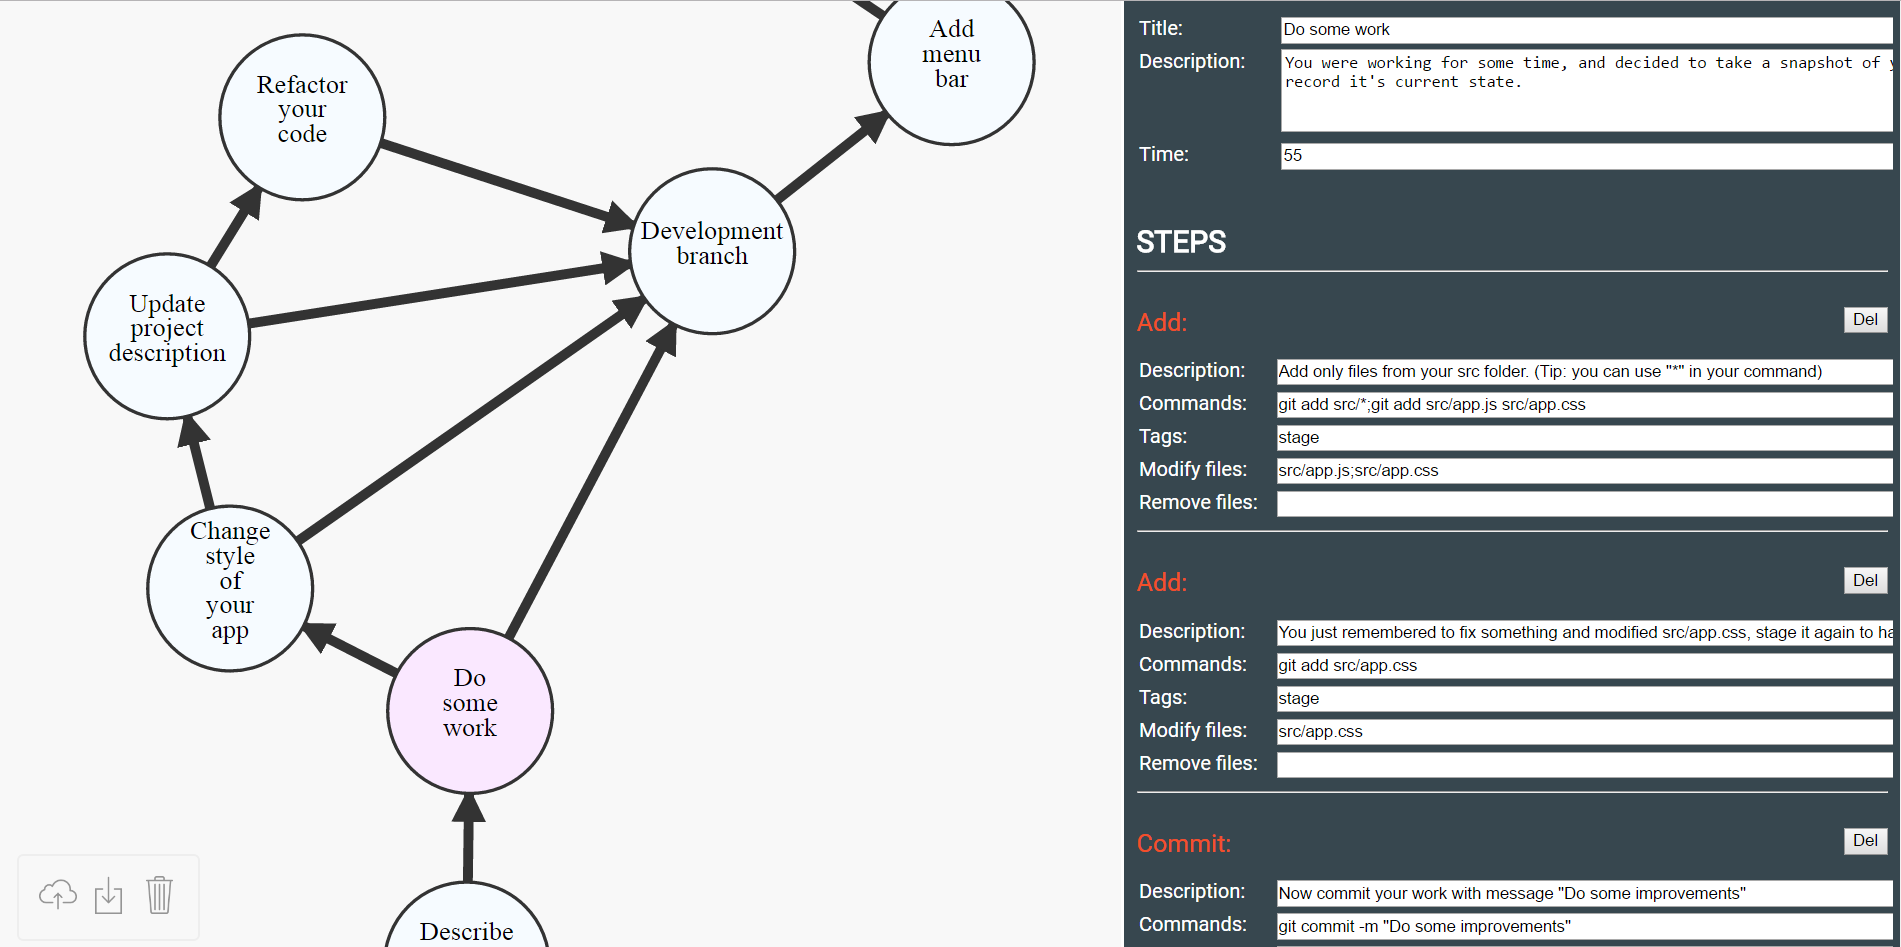
\includegraphics[height=7.5cm]{taskCreator01}
		\caption{Interfejs graficzny narzędzia TaskCreator}
		\label{fig:taskCreator}
	\end{figure}

	Aby dodać nowy węzeł grafu należy przytrzymać klawisz Shift i kliknąć myszką w~wybrane miejsce. Żeby edytować wierzchołek należy go~wybrać poprzez kliknięcie. Z~kolei przytrzymanie klawisza Shift oraz wciśniętego lewego przycisku myszki, a~następnie przeciągniecie kursora znad jednego węzła na drugi, utworzy skierowaną krawędź między nimi. Aby usunąć wybrany wierzchołek grafu bądź jego krawędź, należy go zaznaczyć kliknięciem oraz nacisnąć klawisz Delete.

	Stworzony w ten sposób graf zadań można zapisać do formatu JSON. W~tym~celu wystarczy kliknąć drugi przycisk w~lewym dolnym rogu ekranu. Narzędzie wygeneruje strukturę grafu zrozumiałą dla aplikacji GITar Hero, określi zadanie inicjujące rozgrywkę i~zapisze dane do pliku \textit{taskGraph.json}. Zapisane w ten sposób grafy można wczytać ponownie do aplikacji TaskCreator naciskając pierwszy przycisk w~lewym dolnym rogu ekranu i~wybierając plik do wczytania.

	\section{Stan i jego tranzycje}

	\subsection{Wstęp}

	Stan naszej aplikacji został podzielony na siedem głównych części. Dla każdej z~nich zdefiniowany został tzw. \textit{reducer} (więcej w sekcji \ref{Redux}) odpowiedzialny za tranzycje stanu w~zależności od typu akcji. Stan jest zatem obiektem posiadającym siedem kluczy, pod którymi zdefiniowane są obiekty definiujące stany określonych części aplikacji.

	Przy implementacji \textit{reducerów} zdecydowano się na popularny wzorzec wykorzystujący instrukcję \textit{switch}, sprawdzającą typ wyemitowanej akcji. Domyślnie zwracany jest niezmieniony fragment stanu, przekazany w pierwszym argumencie funkcji. Za pomocą słowa kluczowego \textit{case} zdefiniowane są natomiast wszystkie przypadki, w~których \textit{reducer} powinien zareagować wygenerowaniem nowego stanu.

	Zgodnie z wytycznymi twórców biblioteki \textit{Redux}, obiekt nowego stanu nie może być zmodyfikowanym obiektem poprzedniego stanu (stan powinien być stały i~nie podlegać mutacjom). Aby uzyskać taki efekt, posłużono się funkcją \textit{cloneDeep} z~pakietu \textit{lodash}, będącego zestawem pomocniczych funkcji służących do operacji na strukturach danych w JavaScript. Funkcja ta przyjmuje na wejściu obiekt, a~zwraca jego głęboką kopię. Jeżeli zatem stan wymaga tranzycji, to najpierw generowana jest jego głęboka kopia, a następnie jest modyfikowana i~zwracana jako nowy stan.

	\subsection{Zadania}

	Część stanu dotycząca zadań informuje przede wszystkim o aktualnym zadaniu wraz z~jego właściwościami. Dodatkowo zapamiętuje czas rozpoczęcia aktualnego zadania, co pozwala na obliczenie nagrody punktowej po wykonaniu go. Dostępna jest również informacja o powodzeniach i~niepowodzeniach w rozwiązywaniu zadań dotyczących określonych poleceń systemu Git. Na jej podstawie wybierane jest później kolejne zadanie, które będzie musiał rozwiązać użytkownik. Informacja o postępach gracza jest także wykorzystywana na końcu gry, do stworzenia statystyk.

	Poniżej opisane zostały akcje, które powodują wygenerowanie nowego stanu.

	\begin{description}
	\item[Nowa poprawna komenda z konsoli] \hfill \\
	Wyemitowanie akcji tego typu następuje na skutek poprawnego wykonania kroku zadania. W~rezultacie kolejny krok ustawiany jest w stanie jako aktywny oraz dodawana jest do statystyk informacja o poprawnie wykonanej komendzie danego rodzaju.
	\item[Nowa niepoprawna komenda z konsoli] \hfill \\
	Akcja tego typu zostanie wyemitowana, kiedy zostało zatwierdzone polecenie w konsoli, które nie należy do dozwolonych komend dla aktywnego kroku. W~efekcie w~stanie pojawi się informacja o~niepoprawnej próbie użycia polecenia danego typu.
	\item[Ostatni podpunkt zadania został wykonany] \hfill \\
	Wywoływana gdy dane zadanie zostało ukończone, czyli gdy ostatni krok został prawidłowo rozwiązany. \textit{Reducer} zareaguje wtedy wygenerowaniem nowego aktywnego zadania na podstawie przechowywanych statystyk dotyczących znajomości poleceń.
	\end{description}

	\subsection{Pomoc} \label{PomocStan}

	Osobną część stanu stanowią informacje dotyczące zakładki pomocy, dostępnej w~dolnej części strony. Pierwszą właściwość stanowi zmienna boolowska określająca, czy zakładka jest aktualnie otwarta, czy zamknięta (\textit{isOpen}). Druga właściwość informuje o~aktywnej sekcji pomocy, widocznej o~ile zakładka jest otwarta (\textit{selectedTab}). Pod ostatnim kluczem (\textit{info}) znajduje się zmienna boolowska stanowiąca o~wyświetleniu dodatkowej informacji dla gracza.

	Akcje, które powodują tranzycję stanu zakładki pomocy to:

	\begin{description}
	\item[Akcja otwarcia zakładki pomocy] \hfill \\
	Emitowana po wpisaniu słowa kluczowego "\textit{help}" w konsoli i zatwierdzeniu klawiszem \textit{Enter} lub kliknięcie informacji wyświetlanej nad konsolą. W wyniku jej wykonania \textit{reducer} ustawia flagę \textit{isOpen} na wartość \textit{true}, natomiast flagę \textit{info} na~wartość \textit{false}. W efekcie zakładka pomocy otwiera się, a~informacja dodatkowa znika.

	\item[Akcja zamknięcia zakładki pomocy] \hfill \\
	Wywoływana przez kliknięcie poza zakładką pomocy, kliknięcie w konsolę, wciśnięcie klawisza \textit{ESC} lub wciśnięcie klawisza \textit{Enter}. \textit{Reducer} otrzymując akcję tego typu ustawia pole~\textit{isOpen} na wartość~\textit{false}, co~skutkuje zamknięciem pomocy.

	\item[Akcja wyboru sekcji pomocy] \hfill \\
	Akcja tego typu informuje o wyborze aktywnej sekcji pomocy. Jest ona emitowana po kliknięciu w~jeden z tytułów sekcji w~nawigacji zakładki. Skutkuje ustawieniem właściwości \textit{selectedTab} na konkretną wartość, przekazaną w danych akcji.

	\item[Akcje nawigacji po sekcjach pomocy] \hfill \\
	Są to akcje przełączenia sekcji pomocy na poprzednią bądź następną. Naturalnie \textit{reducer} reaguje zmianą stanu pola dotyczącego aktywnej sekcji, ustawiając je na wartość poprzednią lub następną względem bieżącej.

	\item[Akcja wyświetlenia dodatkowej informacji] \hfill \\
	Akcja ta emitowana jest kiedy pojawia się zadanie nowego typu (dotyczące nowego zagadnienia). Efektem jej wywołania jest ustawienie wartości \textit{true} w~polu~\textit{info} oraz ustawienie odpowiedniej sekcji pomocy.
	\end{description}

	\subsection{Drzewo plików} \label{DrzewoStan}

	Aby symulować modyfikacje na plikach w repozytorium kontrolowanym przez gracza, potrzebna była reprezentacja tychże plików jako części stanu aplikacji. Struktura ta jest rekursywna i~umożliwia dowolne zagnieżdżanie plików w~katalogach. Każdy katalog jest reprezentowany przez obiekt, posiadający nazwę oraz zawartość w~formie tablicy obiektów. Pliki, również reprezentowane przez obiekty, zawierają obowiązkowo nazwę, ale także pola statusu oraz typu zmiany (nie posiadają pola zawartości). Część stanu reprezentująca katalog główny jest zatem tablicą obiektów o strukturze opisanej powyżej.

	Akcje, powodujące tranzycję stanu drzewa plików zostały opisane poniżej.

	\begin{description}
	\item[Akcja modyfikacji drzewa plików] \hfill \\
	Akcja ta została przygotowana, aby móc swobodnie operować na drzewie plików. We właściwościach akcji określane są pliki, które zostaną usunięte, zmodyfikowane lub dodane. \textit{Reducer} reaguje operacjami na strukturze reprezentującej drzewo plików dodając, usuwając i~modyfikując odpowiednie węzły.

	\item[Akcja zatwierdzenia poprawnej komendy w konsoli] \hfill \\
	Pliki w repozytorium zmieniają swoje statusy w~wyniku utworzenia nowej rewizji lub dodania plików do indeksu. W~związku z~faktem, że każdy \textit{reducer} informowany jest o~każdej wyemitowanej akcji, można w łatwy sposób stwierdzić żądanie utworzenia rewizji lub zaindeksowania plików z~poziomu \textit{reducera}. Wystarczy, że~po~otrzymaniu akcji zatwierdzenia w~konsoli poprawnej komendy sprawdzona zostanie składnia tego polecenia. Jeżeli odpowiada ona składni dodawania rewizji lub indeksowania zmian, \textit{reducer} wygeneruje nowy stan, odpowiadający drzewu plików z nowymi statusami. W przeciwnym wypadku zwrócony zostanie niezmieniony stan.
	\end{description}

	\subsection{Punkty}

	Część stanu dotycząca punktów zawiera informację o aktualnej liczbie punktów zdobytych przez gracza.

	\textit{Reducer} odpowiedzialny za stan punktów reaguje wygenerowaniem nowego stanu tylko w przypadku dwóch typów akcji:

	\begin{description}
	\item[Akcja wykonania ostatniego kroku zadania] \hfill \\
	W~takim przypadku liczony jest najpierw ułamek informujący o~tym, jaka część czasu przeznaczonego na zadanie została wykorzystana (czas przydzielony do zadania jest liniowo zależny od liczby jego kroków). Następnie na podstawie tego stosunku i~maksymalnej liczby punktów, możliwych do uzyskania za to zadanie, wyliczana jest nagroda punktowa. Ostatnim krokiem jest dodanie otrzymanej nagrody do aktualnego wyniku i~zwrócenie nowego stanu.

	\item[Akcja zatwierdzenia niepoprawnej komendy] \hfill \\
	Zgodnie z założeniami, wpisanie niepoprawnej komendy skutkuje przyznaniem punktów ujemnych. Po wywołaniu tej akcji, \textit{reducer} odejmuje określoną liczbę punktów od aktualnej wartości i zwraca nowy stan.
	\end{description}

	\subsection{Tutorial} \label{TutorialStan}

	Podczas pierwszego uruchomienia aplikacji gracz zostanie zapoznany z~zasadami gry przez wiadomości pojawiające się w~odpowiednich miejscach ekranu. Wyjaśniają one do czego służą poszczególne elementy interfejsu i~tłumaczą jak prawidłowo z~nich korzystać. Każda z takich wiadomości ma swój identyfikator. Stan przechowuje identyfikator aktualnie wyświetlanej wiadomości (lub wartość \textit{undefined}, gdy nie jest wyświetlana żadna wiadomość).

	Zostały przygotowane cztery wiadomości wprowadzające. \textit{Reducer} ma dostęp do tablicy \textit{tutorialsQueue}, w której zapisane są identyfikatory wiadomości zgodnie z~kolejnością ich wyświetlania. \textit{Reducer} generuje nowy stan w przypadku wyemitowania akcji informującej o~zamknięciu wiadomości. Zmienna \textit{current}, określająca aktualnie wyświetlaną wiadomość, zmienia się wtedy na wartość następną w~stosunku do~aktualnej w~tablicy \textit{tutorialsQueue}. W~efekcie akcja zamknięcia wiadomości w~przypadku pierwszych trzech powoduje przełączenie aktualnej wiadomości na~kolejną. Zamknięcie ostatniej wiadomości ustawia wartość zmiennej \textit{current} na~\textit{undefined}, co~oznacza, że~\textit{tutorial} został ukończony.

	\subsection{Konsola}

	Konsola posiada wbudowany mechanizm autouzupełniania, imitujący zachowanie znane z konsoli systemowej. Kluczowa dla działania mechanizmu jest znajomość nazw gałęzi utworzonych w repozytorium. W tym celu utworzono \textit{reducer}, który reaguje na akcję zatwierdzenia poprawnej komendy. Jeżeli komenda ta powoduje utworzenie nowej gałęzi repozytorium, jej nazwa jest zapisywana w tablicy \textit{branches}, w części stanu aplikacji dostępnej pod kluczem \textit{console}. Tablica ta jest później wykorzystywana do stworzenia drzewa autouzupełniania (patrz \ref{KonsolaKomponent}).

	\subsection{Podsumowanie}

Zgodnie z~założeniami projektu, gracz może ocenić swój postęp na~podstawie punktacji oraz statystyk. Obie wartości są przechowywane w stanie. Aby wyświetlić podsumowanie, potrzebna jest jednak informacja o~zakończeniu rozgrywki. W~tym celu wydzielono część stanu dostępną pod kluczem \textit{summary}. Zawiera ona jedną zmienną boolowską \textit{show} informującą o wyświetlaniu lub ukryciu podsumowania. Zaimplementowano również \textit{reducer}, reagujący na wywołanie akcji wykonania ostatniego zadania. Ustawia on wtedy flagę \textit{show} na wartość \textit{true}, co skutkuje wyświetleniem podsumowania.

	\section{Komponenty graficzne}

	\subsection{Wstęp}

	Do połączenia komponentów interfejsu ze stanem aplikacji wykorzystano specjalny komponent \textit{Connect}, przygotowany przez twórców biblioteki \textit{Redux}. Pozwala on na~przekazanie konkretnych właściwości stanu do komponentu użytkownika. W~celu strukturyzacji projektu zdecydowano się wydzielić komponenty połączone ze stanem do osobnego katalogu. Jest to praktyka popularna wśród twórców aplikacji opartych o \textit{React} i~\textit{Redux}. Komponenty takie będą dalej nazywane kontenerami.

	\subsection{Komponenty pomocnicze} \label{KomponentyPomocnicze}

	W celu zwiększenia modułowości projektu oraz jednokrotnej implementacji powtarzających się funkcjonalności zaimplementowano sześć komponentów pomocniczych, które zostały opisane poniżej.

	\begin{description}
	\item[Komponent rozmywający] \hfill \\
	Niektóre stany aplikacji, jak na przykład wprowadzenie do gry czy korzystanie z zakładki pomocy, wymagają od gracza chwilowego skupienia uwagi na wyszczególnionym elemencie ekranu. W tym celu zaimplementowano pomocniczy komponent \textit{Blur}, służący nałożeniu na wybrany element graficzny filtra rozmywającego. Element docelowy przekazywany jest jako zawartość komponentu \textit{Blur}. Za pomocą właściwości \textit{blur} można określić, czy ma zostać użyty filtr rozmywający, natomiast właściwość \textit{active} określa, czy element ma reagować na zdarzenia myszy.

	\item[Checkbox] \hfill \\
	Pole symbolizujące wykonanie lub niewykonanie danego kroku jest potrzebne do wyświetlenia listy kroków aktualnego zadania. Komponent przyjmuje trzy parametry wejściowe:

	\begin{itemize}
		\item \textit{value} - zmienna boolowska określająca, czy pole jest zaznaczone,
		\item \textit{active} - zmienna boolowska określająca, czy pole jest aktywne (w~praktyce oznacza to użycie jaśniejszego koloru),
		\item \textit{size} - parametr opcjonalny, określający wysokość i szerokość pola.
	\end{itemize}

	W przyszłości element ten może być wykorzystany również jako pole formularza typu \textit{checkbox}.

	\item[Ładowanie] \hfill \\
	Podczas rozgrywki istnieją sytuacje, w~których należy zasygnalizować graczowi oczekiwanie na~pewien typ zdarzenia. Przykładem jest stan, w~którym wykonywane są zmiany w~plikach repozytorium, a gracz oczekuje na krok dotyczący dodania zmian do indeksu. W tym celu zaimplementowano komponent \textit{Loader} przedstawiający trzy kropki animowane za pomocą arkuszy \textit{CSS}.

	\item[Licznik] \hfill \\
	Zmiana aktualnej liczby punktów po wykonaniu ostatniego kroku zadania jest natychmiastowa. Aby zwiększyć atrakcyjność graficzną aplikacji, zdecydowano się na dodanie animacji płynnej zmiany liczby punktów w~komponencie. W~tym celu zaimplementowano pomocniczy komponent licznika, który w~swoim wewnętrznym stanie przechowuje aktualnie wyświetlaną liczbę. Za~pomocą metody \textit{componentWillReceiveProps} otrzymuje on informację o~zmianie liczby punktów w~stanie aplikacji. Zmiana faktycznie wyświetlanej liczby jest wykonywana co klatkę, interpolując czas, który upłynął od początku animacji na~liczbę punktów. Ostatecznie, po czasie określonym jako czas animacji, wartość jest ustawiana na~docelową.

	\item[Plik] \hfill \\
	W kilku miejscach aplikacji wymagane jest wyświetlenie obiektu symbolizującego plik repozytorium. Zaimplementowany został komponent, przyjmujący jako parametry nazwę pliku oraz jego status. Dzięki użyciu komponentu, wszystkie obiekty graficzne reprezentujące pliki w aplikacji wyglądają tak samo.
	
	\item[Panel] \hfill \\
	Do wyświetlania wiadomości wprowadzających, opisów zadań oraz podsumowania zdefiniowany został komponent \textit{Panel}. Przyjmuje on jeden opcjonalny argument \textit{title} określający tytuł wiadomości. Treść wiadomości
przekazywana jest jako zawartość komponentu. Pozwala to na wyświetlanie dowolnych elementów \textit{HTML} lub innych komponentów we wnętrzu wiadomości.
	\end{description}

	\subsection{Tutorial}
	W celu wyświetlenia wprowadzenia, pojawiającego się po uruchomieniu aplikacji, zaimplementowany został kontener \textit{Tutorial}. Korzysta on z właściwości \textit{tutorial.current} stanu aplikacji, określającej aktualnie wyświetlaną wiadomość wprowadzającą. W~wydzielonym pliku zostały zdefiniowane cztery wiadomości, każda z nich ma określoną treść i pozycję na ekranie. Jeżeli istnieje wśród nich wiadomość odpowiadająca aktualnej wartości stanu, to zostanie ona wyświetlona przez kontener \textit{Tutorial}.

	\begin{figure}[h]
		\centering
		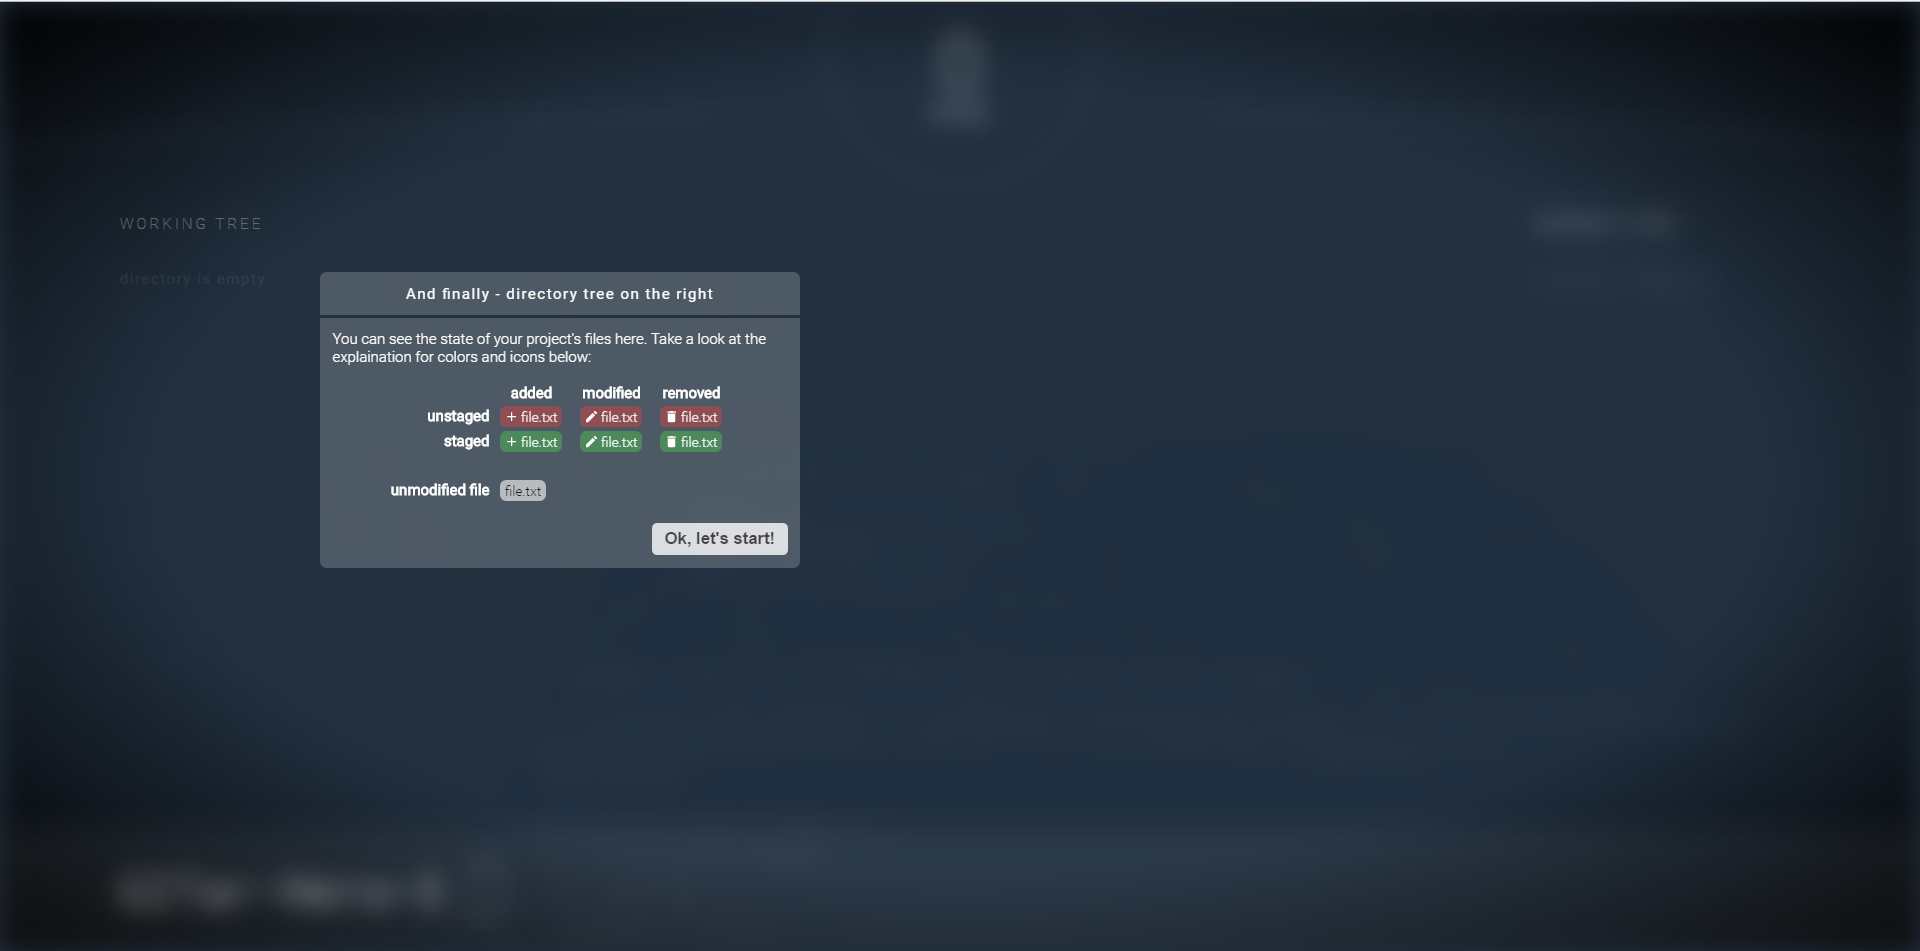
\includegraphics[width=15cm]{component-tutorial}
		\caption{Wiadomość tutoriala prezentująca drzewo plików}
		\label{fig:tutorial}
	\end{figure}
	\FloatBarrier

	\subsection{Kontener aplikacji}

	Kontener aplikacji (\textit{App}) stanowi korzeń drzewa komponentów interfejsu graficznego. Oznacza to, że jest on odpowiedzialny za~wyrenderowanie całego widoku aplikacji, wywołuje zatem wszystkie pozostałe komponenty. Cała zawartość kontenera zamknięta jest w~komponencie \textit{Provider}. Jest on dostarczony wraz z biblioteką \textit{Redux}, a~jego użycie jest wymagane dla poprawnego jej działania.

	Kontener \textit{App} nie tylko wywołuje pozostałe komponenty, ale również zarządza nakładaniem na nie filtra rozmywającego (korzystając z komponentu pomocniczego \textit{Blur}). Jest to możliwe dzięki połączeniu kontenera z właściwościami stanu dotyczącymi wprowadzenia, zakładki pomocy oraz podsumowania i przekazaniu odpowiednich parametrów wejściowych do instancji komponentu \textit{Blur}.

	\subsection{Aktualne zadanie}

	Aktualne zadanie (\textit{CurrentTask}) jest kontenerem korzystającym z części stanu aplikacji dotyczącej zadań. Jego rolą jest wyświetlanie aktualnego zadania, wraz ze~wszystkimi jego krokami. W~pierwszej kolejności komponent pobiera z listy zadań aktualne zadanie. Przy pomocy komponentu pomocniczego \textit{Panel}, wyświetlany jest tytuł i~opis zadania. Lista kroków korzysta natomiast z komponentu pomocniczego \textit{Checkbox}. Dodatkowo wykorzystany został tutaj komponent pomocniczy, napisany przez twórców biblioteki \textit{React}, a~mianowicie \textit{ReactCSSTransitionGroup}. Dzięki umieszczeniu elementu HTML zawierającego zadanie w~komponencie \textit{ReactCSSTransitionGroup} możliwe jest zdefiniowanie jego animacji wejścia i~wyjścia przy pomocy arkuszy stylów \textit{CSS}.

	\begin{figure}[h]
		\centering
		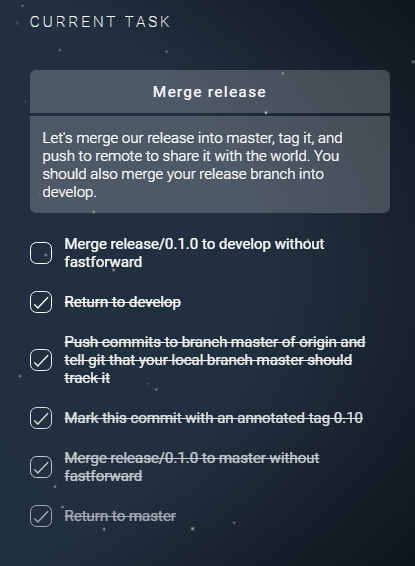
\includegraphics[height=6.1cm]{component-task}
		\caption{Komponent zawierający aktualne zadanie}
		\label{fig:task-list}
	\end{figure}
	\FloatBarrier
	\subsection{Konsola} \label{KonsolaKomponent}

	Konsola jest komponentem przyjmującym na wejściu cztery parametry. Pierwszy z~nich (\textit{enabled}) daje możliwość zablokowania konsoli, np.~w~przypadku, gdy tutorial nie został jeszcze ukończony. Kolejne dwa parametry (\textit{files}, \textit{branches}) to tablice wartości tekstowych, z~nazwami istniejących w~repozytorium plików oraz gałęzi. Nazwy te są potrzebne do działania funkcji autouzupełniania, znanej z~konsolowej wersji programu Git. Ostatni argument (\textit{onCommandEnter}) jest funkcją, która będzie wywołana, kiedy w~konsoli zostanie zatwierdzona komenda.

	Komponent konsoli wykorzystuje element \textit{input}, czyli pole tekstowe formularza \textit{HTML}. Niestety, właściwości \textit{CSS} mają ograniczony wpływ na wygląd takiego pola. W~związku z~tym zmiany w~tym polu śledzone są przy pomocy zdarzenia \textit{onChange}, a~sam element jest renderowany jako przezroczysty. Po każdej zmianie wartości elementu \textit{input} jego wartość zostaje przepisana do innego elementu \textit{HTML}, który dzięki użyciu elementów pomocniczych oraz arkuszy \textit{CSS} przypomina wyglądem konsolę systemową.

	\begin{figure}[h]
		\centering
		
\includegraphics[width=15cm]{component-console}
		\caption{Konsola do wpisywania poleceń}
		\label{fig:console}
	\end{figure}

	Dodatkowo, aby upodobnić komponent do konsoli znanej z systemów operacyjnych, możliwe jest korzystanie z historii wpisywanych komend. Efekt ten osiągnięty został dzięki zapisywaniu każdego wprowadzanego polecenia w~stanie komponentu. Aby podnieść walory wizualne komponentu, historia jest czasowo wyświetlona nad obszarem wpisywania podczas używania klawiszy strzałek górnej i~dolnej.

	Dla ułatwienia szybkiej rozgrywki zaimplementowano mechanizm autouzupełniania dla nazw plików oraz gałęzi repozytorium. Wymagało to w~pierwszej kolejności zaprojektowania struktury drzewa podpowiedzi. Struktura ta opiera się na obiektach, z~których każdy posiada obowiązkowo właściwość \textit{pattern} oraz opcjonalnie właściwość \textit{children}. Pierwsza z~nich określa ciąg znaków, do których dopasowuje się dany węzeł drzewa oraz wszystkie jego następniki. Druga natomiast, o~ile jest zdefiniowana, przechowuje tablicę następników węzła.

	Zaimplementowano funkcje pomocnicze służące do generowania i~przeszukiwania drzewa autouzupełniania. Pierwsza z~nich umożliwia budowanie drzew autouzupełniania na podstawie wzoru zawierającego określone słowo kluczowe. Przykładowo, dla~wartości \textit{,,git checkout :branch:''} oraz tablicy wartości tekstowych, zawierającej nazwy istniejących gałęzi, wygenerowane zostanie drzewo autouzupełniania biorące pod uwagę polecenie tekstowe ,,\textit{git checkout}'' oraz listę gałęzi (z~uwzględnieniem możliwości nakładania się na siebie ich nazw). Mając do~dyspozycji listę dostępnych komend (w~odpowiedniej składni), listę istniejących gałęzi oraz plików, dzięki tej funkcji można zbudować drzewo, pozwalające w~dużym stopniu zasymulować autouzupełnianie znane z~konsoli systemowej. Funkcja przeszukująca dostaje na wejściu ciąg znaków (aktualną zawartość konsoli). Rozpoczynając od korzenia drzewa przechodzi w~kierunku liści, szukając węzła, którego wzór zawiera wejściowy ciąg znaków. Jeżeli taki węzeł zostanie znaleziony, to~jego wzór jest zwracany jako podpowiedź.

	Generowanie drzewa podpowiedzi jest stosunkowo kosztowną operacją, dlatego wykonywana jest ona tylko jeżeli zmieniła się lista plików lub gałęzi. Przeszukiwanie odbywa się za~każdym razem, gdy~podczas używania konsoli wciśnięty zostanie klawisz tabulacji.

	\subsection{Pomoc}

	Zakładka pomocy jest kontenerem zawierającym komponent konsoli oraz treść materiałów dydaktycznych i~wskazówek przydatnych podczas rozwiązywania zadań. Kontener korzysta z~czterech właściwości stanu aplikacji:
	\begin{itemize}
		\item drzewa plików - potrzebnego do przekazania listy istniejących w~repozytorium plików do komponentu konsoli,
		\item aktywnej wiadomości tutoriala - wymaganej do uniemożliwienia interakcji z~konsolą do czasu zakończenia tutoriala,
		\item stanu zakładki pomocy - służącej do odpowiedniego wystylizowania zakładki w zależności od tego, czy jest otwarta, czy zamknięta,
		\item stanu konsoli - w celu przekazania do komponentu konsoli listy gałęzi repozytorium.
	\end{itemize}

	\begin{figure}[h]
		\centering
		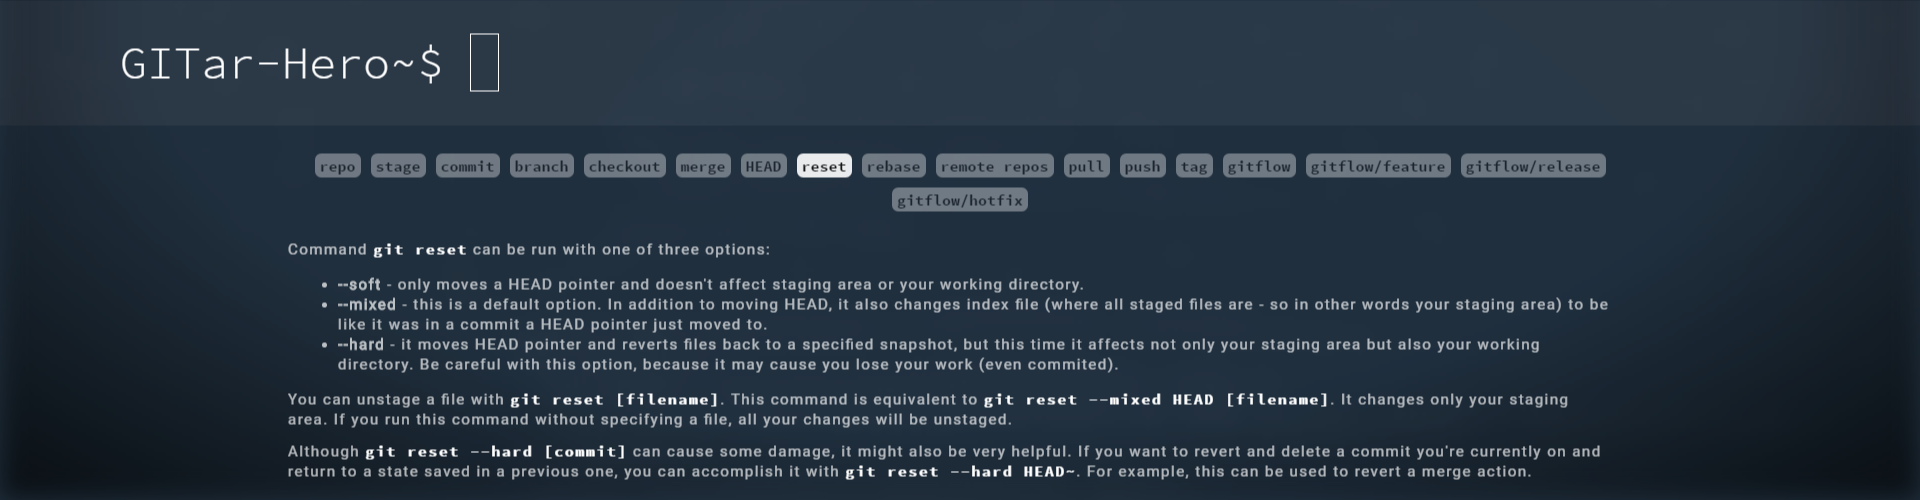
\includegraphics[width=15cm]{component-help}
		\caption{Zakładka pomocy z otwartą sekcją ,,\textit{reset}''}
		\label{fig:help-drawer}
	\end{figure}

	Gdy zakładka jest otwarta, wysuwa się z dolnej części ekranu spod konsoli. Efekt ten został osiągnięty przez animowanie właściwości \textit{translateY} elementu, które jest wysoce wydajne, ponieważ jest wykonywane na~karcie graficznej (w~odróżnieniu od właściwości takich jak \textit{top}, czy \textit{margin-top}, które pozwalałyby osiągnąć podobny efekt). Z zakładką pomocy związane są także animacje wywoływane podczas zmiany aktualnie wyświetlanej sekcji.

	Kontener pomocy emituje akcje związane ze zmianami stanu zakładki pomocy (patrz:~\ref{PomocStan}) oraz akcję zatwierdzenia nowej komendy (poprzez przekazanie komponentowi konsoli funkcji emitującej tę akcję).

	\subsection{Drzewo plików}

	Kontener drzewa plików jest odpowiedzialny za wyświetlenie informacji o~strukturze katalogu roboczego, w~którym znajduje się repozytorium. Korzysta on z~części stanu dotyczącej drzewa plików.

	Zaimplementowana została pomocnicza funkcja renderująca \textit{renderRecursively}, umożliwiająca wyświetlenie plików na~dowolnym poziomie zagnieżdżenia. W~jej pierwszym wywołaniu jako argument podawane jest drzewo plików ze~stanu. Ma~ono strukturę tablicy (patrz:~\ref{DrzewoStan}). Dla każdego z~elementów funkcja sprawdza czy jest on plikiem, czy katalogiem. Jeżeli jest to~plik, to~zwrócony zostaje pomocniczy komponent pliku (patrz \ref{KomponentyPomocnicze}). W~przypadku katalogu zwracany jest nowy element \textit{HTML} wyświetlający jego nazwę, a~zawartość folderu wyświetlana jest poprzez rekursywne wywołanie funkcji \textit{renderRecursively}. Dodatkowo, katalogi w których nie ma plików o statusie innym niż "\textit{niezmodyfikowany}" są zwijane, aby ograniczyć wysokość komponentu.

	\begin{figure}[h]
		\centering
		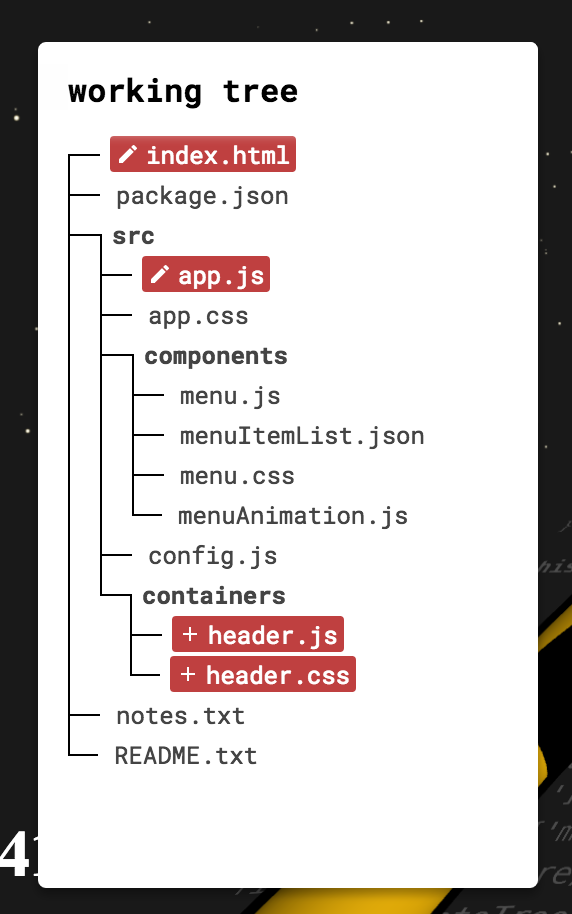
\includegraphics[height=4.4cm]{component-tree}
		\caption{Drzewo plików, wyświetlające aktualny stan obszaru roboczego}
		\label{fig:tree}
	\end{figure}
	\FloatBarrier

	\subsection{Czas, punkty, postęp}

	Zaimplementowano zbiorczy kontener wyświetlający komponenty w~górnej części widoku. Do wyświetlenia aktualnej liczby punktów posłużono się komponentem pomocniczym \textit{Licznik} (patrz: \ref{KomponentyPomocnicze}). Przy pomocy dynamicznie generowanego elementu \textit{SVG}, udało się stworzyć linie postępu, symbolizujące wykonaną część aktualnego zadania. Podobnie jak w przypadku komponentu licznika, aktualnie wyświetlana wartość postępu jest przechowywana w wewnętrznym stanie komponentu~i~animowana przy pomocy funkcji \textit{requestAnimationFrame} udostępnianej przez przeglądarkę.

	Podobnie, wykorzystując element \textit{SVG}, renderowany jest element przypominający prędkościomierz. Reprezentuje on czas przeznaczony na wykonanie zadania. Dynamiczne generowanie elementu pozwala na ustawienie konkretnego koloru dla wybranych linii wartości. Wszystkie linie podświetlają się, gdy pojawia się nowe zadanie i wygaszają się z upływem czasu (prędkość wygaszania zależy od czasu przeznaczonego na zadanie). Ponieważ stan linii wartości zmienia się maksymalnie kilka razy w~ciągu sekundy, nie ma potrzeby użycia funkcji \textit{requestAnimationFrame} i aktualizowania komponentu w każdej klatce. Zamiast tego została użyta funkcja \textit{setInterval}, aktualizująca element w~drzewie \textit{DOM} dziesięć razy na~sekundę.

	\begin{figure}[h]
		\centering
		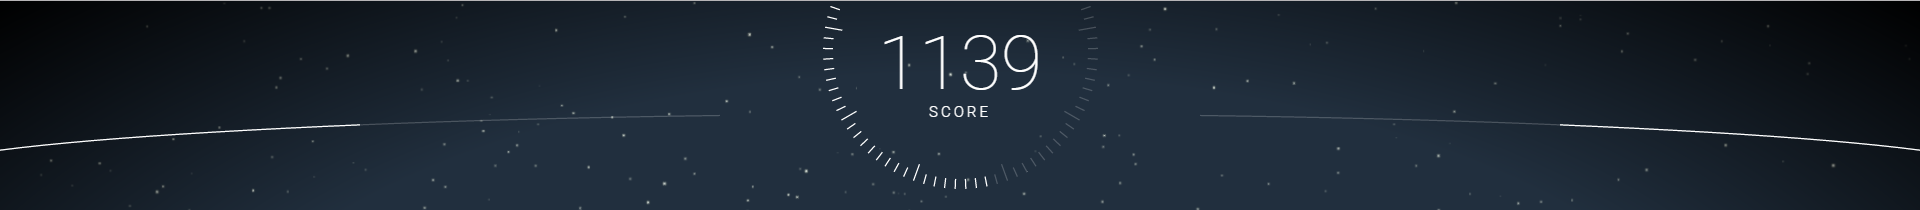
\includegraphics[width=15cm]{component-top}
		\caption{Punkty, pozostały czas oraz linie postępu}
		\label{fig:top}
	\end{figure}

	\subsection{Podsumowanie}

	Podsumowanie jest kontenerem mającym za zadanie wyświetlić wiadomość końcową po wykonaniu przez gracza ostatniego zadania. Pobiera on ze stanu aplikacji informacje o aktualnej liczbie punktów oraz statystyki dotyczące poprawności wpisywanych komend. Wiadomość wyświetlana jest przy pomocy komponentu \textit{Panel}. Statystyki są pokazywane w formie tabeli, dzięki czemu gracz może zobaczyć jak radził sobie z konkretnymi zagadnieniami.

	\begin{figure}[h]
		\centering
		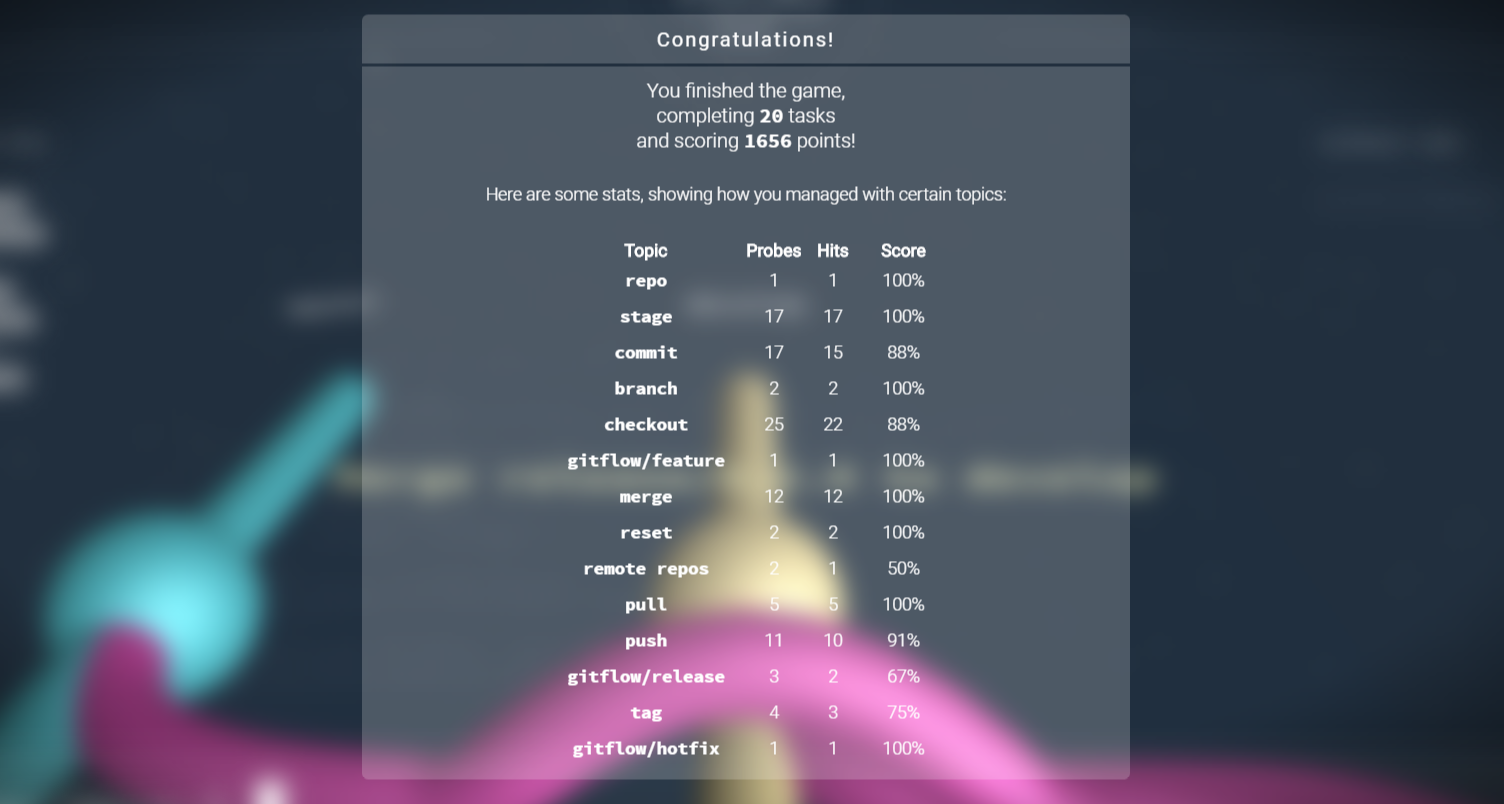
\includegraphics[width=15cm]{component-summary}
		\caption{Podsumowanie zawierające statystyki dotyczące przebiegu gry}
		\label{fig:summary}
	\end{figure}

	\subsection{Canvas}

	Komponent \textit{Canvas} stanowi połączenie między architekturą opartą o~komponenty \textit{React} i~stan aplikacji, a~moduł 3D, zaimplementowany z~wykorzystaniem biblioteki \textit{Babylon.js}.

	Pierwszym zadaniem komponentu jest wstawienie do obiektowego modelu dokumentu elementu \textit{canvas}, który umożliwia rysowanie przy pomocy technologii \textit{WebGL}. Założono dodatkowo, że~po~utworzeniu tego elementu, powinien on~być modyfikowalny tylko z~poziomu modułu 3D (metoda \textit{render} komponentu powinna wykonać się tylko raz). Efekt ten osiągnięto implementując metodę \textit{shouldComponentUpdate} i zwracając w niej zawsze wartość \textit{false}. \textit{React} pozwala na zaimplementowanie tej metody w przypadku, w~którym użytkownik chce zablokować przerysowanie komponentu po zmianie jego stanu lub parametrów wejściowych. Po utworzeniu elementu \textit{canvas}, inicjowany jest moduł 3D, do którego element ten przekazywany jest jako argument.

	Parametrem wejściowym komponentu \textit{Canvas} jest obiekt \textit{store}, zawierający stan aplikacji i~umożliwiający reagowanie na~emitowane akcje. Jest on~wykorzystywany do~przekazywania modułowi~3D informacji o~zmianach, które pojawiły się w~repozytorium.

	\section{Grafika 3D}

	\subsection{Repozytorium 3D}
	W~celu kontrolowania właściwego odwzorowywania stanu repozytorium za pomocą grafiki 3D stworzono obiekt \textit{Repo3D}. Służy on jako kontroler, reagujący na~wprowadzane przez użytkownika komendy i~zarządzający elementami grafiki 3D. Nasłuchuje na wykonywane akcje i~w~zależności od ich typu dodaje, usuwa bądź modyfikuje elementy na scenie. Kontroler \textit{Repo3D} zawiera wszystkie potrzebne informacje dotyczące aktualnego stanu repozytorium, czyli między innymi listę utworzonych gałęzi, zawierane przez nie rewizje oraz wskaźnik HEAD, o którym więcej w podrozdziale~\ref{camera}.

	\subsection{Gałąź}
	Każda gałąź w repozytorium reprezentowana jest przez odpowiedni obiekt 3D nazwany \textit{Branch}. Tworzenie tego obiektu realizowane jest przy pomocy funkcji \textit{CreateTube} z~biblioteki \textit{Babylon.js}. Na~podstawie podanej listy punktów składających się na~ścieżkę funkcja ta generuje siatkę wierzchołków w~kształcie tuby. Pozwala również na podanie średnicy oraz szczegółowości siatki. Parametry te dobrano w taki sposób, aby wygenerować tubę, której przekrój przypomina koło, przy jednoczesnym zachowaniu jak najmniejszej liczby użytych wierzchołków. 

	Jedna gałąź może składać się z dwóch rodzajów siatki. 
	\begin{itemize}
		\item \textbf{Główny człon}~---~reprezentuje podstawową część gałęzi, będącą prostą tubą. Ścieżka użyta do jej wygenerowania zawiera tylko dwa punkty, wyznaczające jej krańce. Dzięki temu można osiągnąć dowolnie długi odcinek, nie zwiększając przy tym liczby wierzchołków.

		\item \textbf{Łącznik gałęzi}~---~wykorzystywany do łączenia dwóch gałęzi. Zostaje utworzony w~momencie dodania do repozytorium nowej gałęzi lub w wyniku wykonania operacji scalania. Do wyznaczenia ścieżki łącznika skorzystano z funkcji pomocniczej, generującej krzywą Beziera. Na podstawie podanych czterech punktów\footnote{Pierwszy z czterech punktów ustala początek krzywej, dwa kolejne służą do określenia kształtu linii, a ostatni definiuje punkt końcowy, czyli punkt początkowy członu innej gałęzi. Dodatkowym parametrem jest liczba wygenerowanych punktów krzywej, wpływającym na szczegółowość linii.} generuje ona tablicę punktów, które tworzą krzywą, określającą kształt łącznika. Następnie sprawdzane jest, czy wygenerowana ścieżka nie przecina istniejącej gałęzi. Jeżeli tak, to podczas tworzenia łącznika odpowiednio zwiększana a~następnie zmniejszana jest wysokość punktów, tak aby łącznik przechodził nad gałęzią.
	\end{itemize}

	Dla gałęzi zaimplementowano animacje wydłużania oraz skracania. Dla głównego członu polega ona na przesunięciu ostatniego punktu ścieżki, a~następnie zaktualizowaniu bufora wierzchołków. Służy do tego ta sama funkcja, co~do~tworzenia początkowej siatki wierzchołków. Jedyna różnica polega na podaniu dodatkowego parametru, którym jest instancja obiektu, którego bufor należy zmienić. 

	W~przypadku łącznika gałęzi animacja jest bardziej skomplikowana, ponieważ rozmiar bufora wierzchołków musi być stały. Oznacza to, że nie można dodawać do niego nowych wierzchołków. W~związku z~tym, aby osiągnąć efekt rozwijania się łącznika, należy wszystkie punkty ścieżki przesunąć na jej początek, a~następnie rozwijać w kierunku końca ścieżki. Analogicznie jak przy animacji głównego członu, po każdej zmianie ścieżki konieczne jest zaktualizowanie bufora wierzchołków.

	\begin{figure}[h]
		\centering
		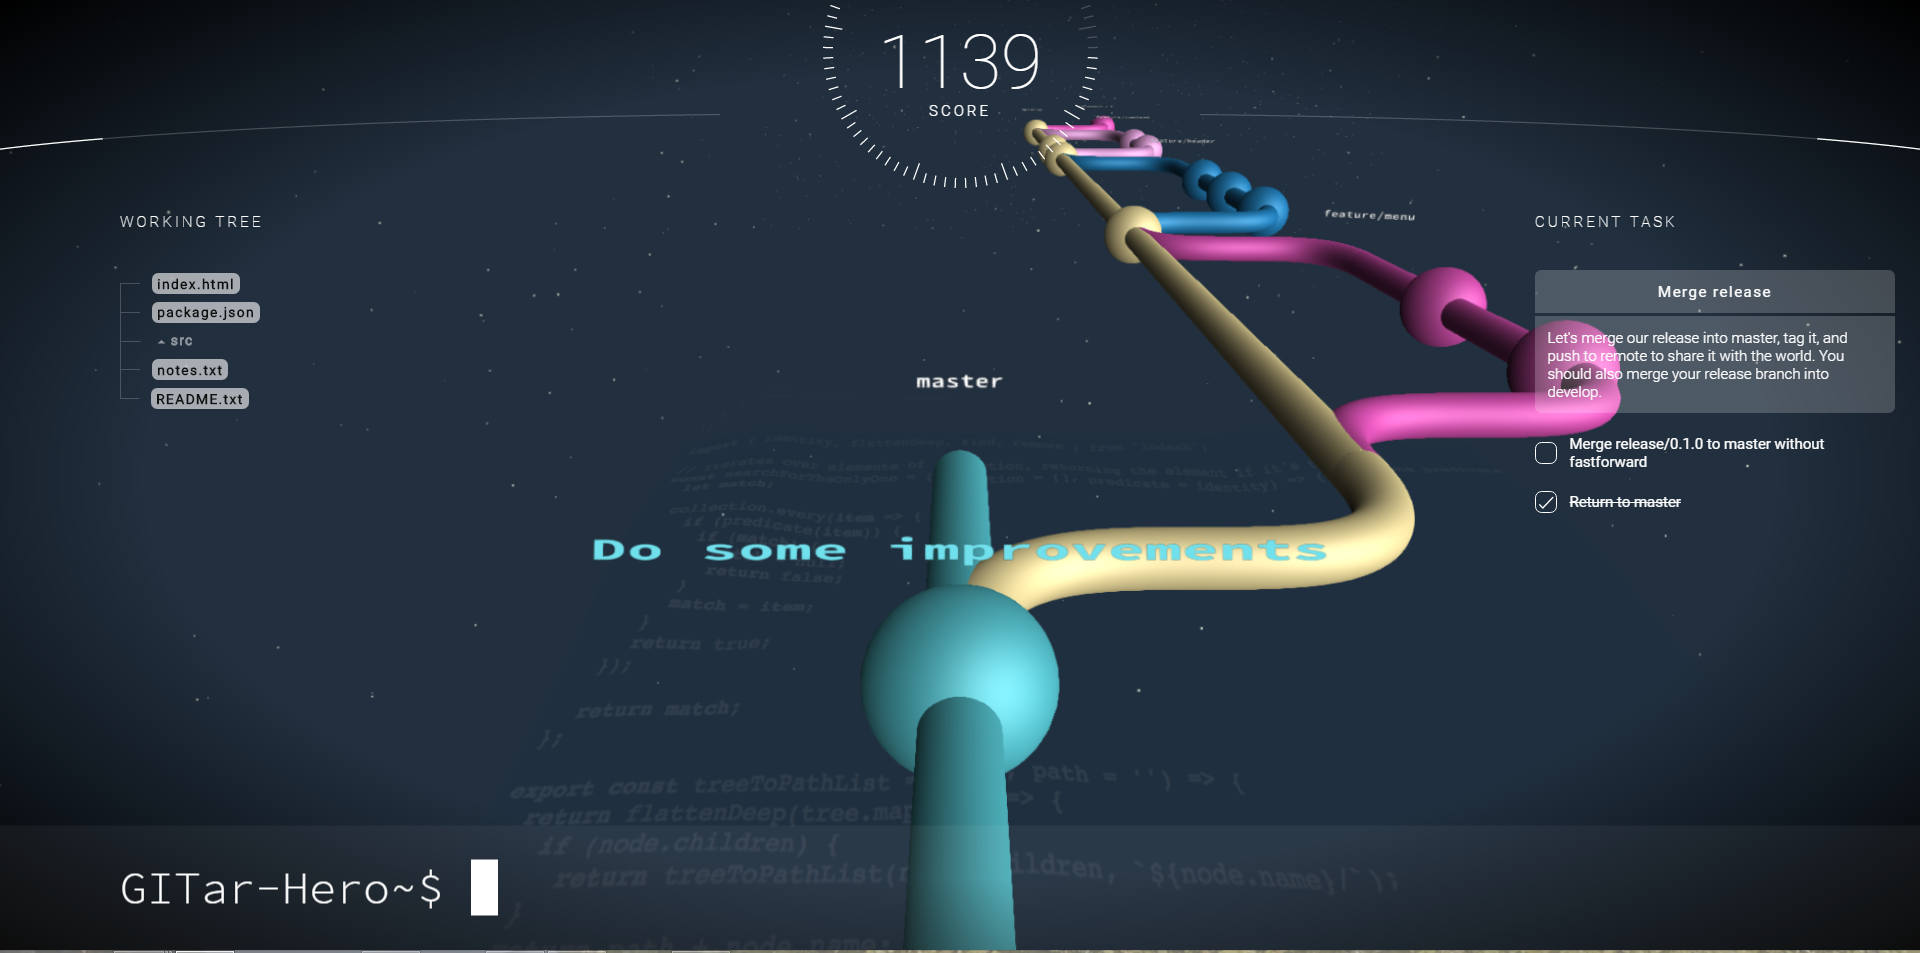
\includegraphics[width=15cm]{branches}
		\caption{Repozytorium zawierające kilka gałęzi, z bieżącą gałęzią \textit{master}}
		\label{fig:branches}
	\end{figure}

	Na gałąź nałożono standardowy materiał. Jest to klasa z biblioteki \textit{Babylon.js} reprezentująca uniwersalny \textit{shader}.  Umożliwia on określenie takich właściwości jak kolor, przezroczystość oraz tekstury.

	Na końcu każdej gałęzi wyświetlany jest tekst, z nazwą gałęzi o~kolorze białym. Jego pozycję ustawiono na~referencję do~ostatniego punktu gałęzi, dzięki czemu tekst zawsze podąża za wydłużającą lub skracającą się gałęzią.

	\subsection{Rewizja}
	Rewizja, powstająca w~wyniku operacji zatwierdzania zmian, w~grafice~3D przedstawiana jest jako obiekt \textit{Commit} o~kształcie kuli. Umieszczona jest na gałęzi, która zawiera daną rewizję.

	Funkcja \textit{CreateSphere} pochodząca z biblioteki \textit{Babylon.js} buduje siatkę wierzchołków w kształcie sfery o~określonej średnicy oraz teselacji. Przy wartości teselacji równej szesnaście powierzchnia obiektu wygląda na wygładzoną.

	Z obiektem \textit{Commit} związany jest napis, zawierający wiadomość podaną przy zatwierdzaniu zmian, który widnieje nad kulą.
	Jego kolor jest nieznacznie jaśniejszy od koloru samego obiektu. \textit{Commit} może poza wiadomością posiadać również etykietę, nadaną poleceniem \textit{git tag}. Etykiety znajdują się nieco powyżej tekstu z~wiadomością. Aby nie wprowadzać zbyt wielu elementów, tekst jest wyświetlany tylko dla tych obiektów \textit{Commit}, które znajdują się na aktywnej aktualnie gałęzi. Podczas przełączania się między gałęziami występuje animacja ukrywająca tekst wszystkich rewizji bieżącej gałęzi oraz ukazująca tekst dotyczący nowej gałęzi.

	Z obiektem ukazującym zatwierdzenie zmian związane są dwie animacje, opisane poniżej.
	\begin{description}
		\item[Powstanie] \hfill \\
		Trwająca niecałe pół sekundy animacja pojawiania się rewizji, polegająca na~modyfikowaniu skali z wykorzystaniem funkcji generującej krzywą Beziera, tak by~przypominało to~sprężanie i~rozprężanie, co tworzy ciekawy efekt wizualny. Animacja występuje gdy tworzona jest nowa rewizja.

		\item[Eksplozja] \hfill \\
		Efektowna animacja z~wybuchem cząsteczek stałych. Do ich utworzenia skorzystano z~wbudowanych mechanizmów biblioteki \textit{Babylon.js}. Na początku tworzona jest figura z kilkuset cząsteczek, będących sferami o tym samym kolorze co obiekt \textit{Commit}. Następnie definiowana jest funkcja wykonywana dla każdej cząsteczki, określająca prędkość oraz kierunek rozchodzenia. W~rezultacie cząsteczki rozchodzą się dynamicznie w~kształcie kuli, a~w~każdej klatce zmniejszana jest ich skala, dzięki czemu maleją i~zanikają. Całość daje efekt eksplozji ciała, co urozmaica doznania wizualne.

		Animacja jest wykonywana kiedy ma zostać usunięta rewizja, czyli gdy użytkownik wykona polecenie resetujące wskaźnik HEAD do wcześniejszej rewizji w repozytorium.
	\end{description}	

	\begin{figure}[h]
		\centering
		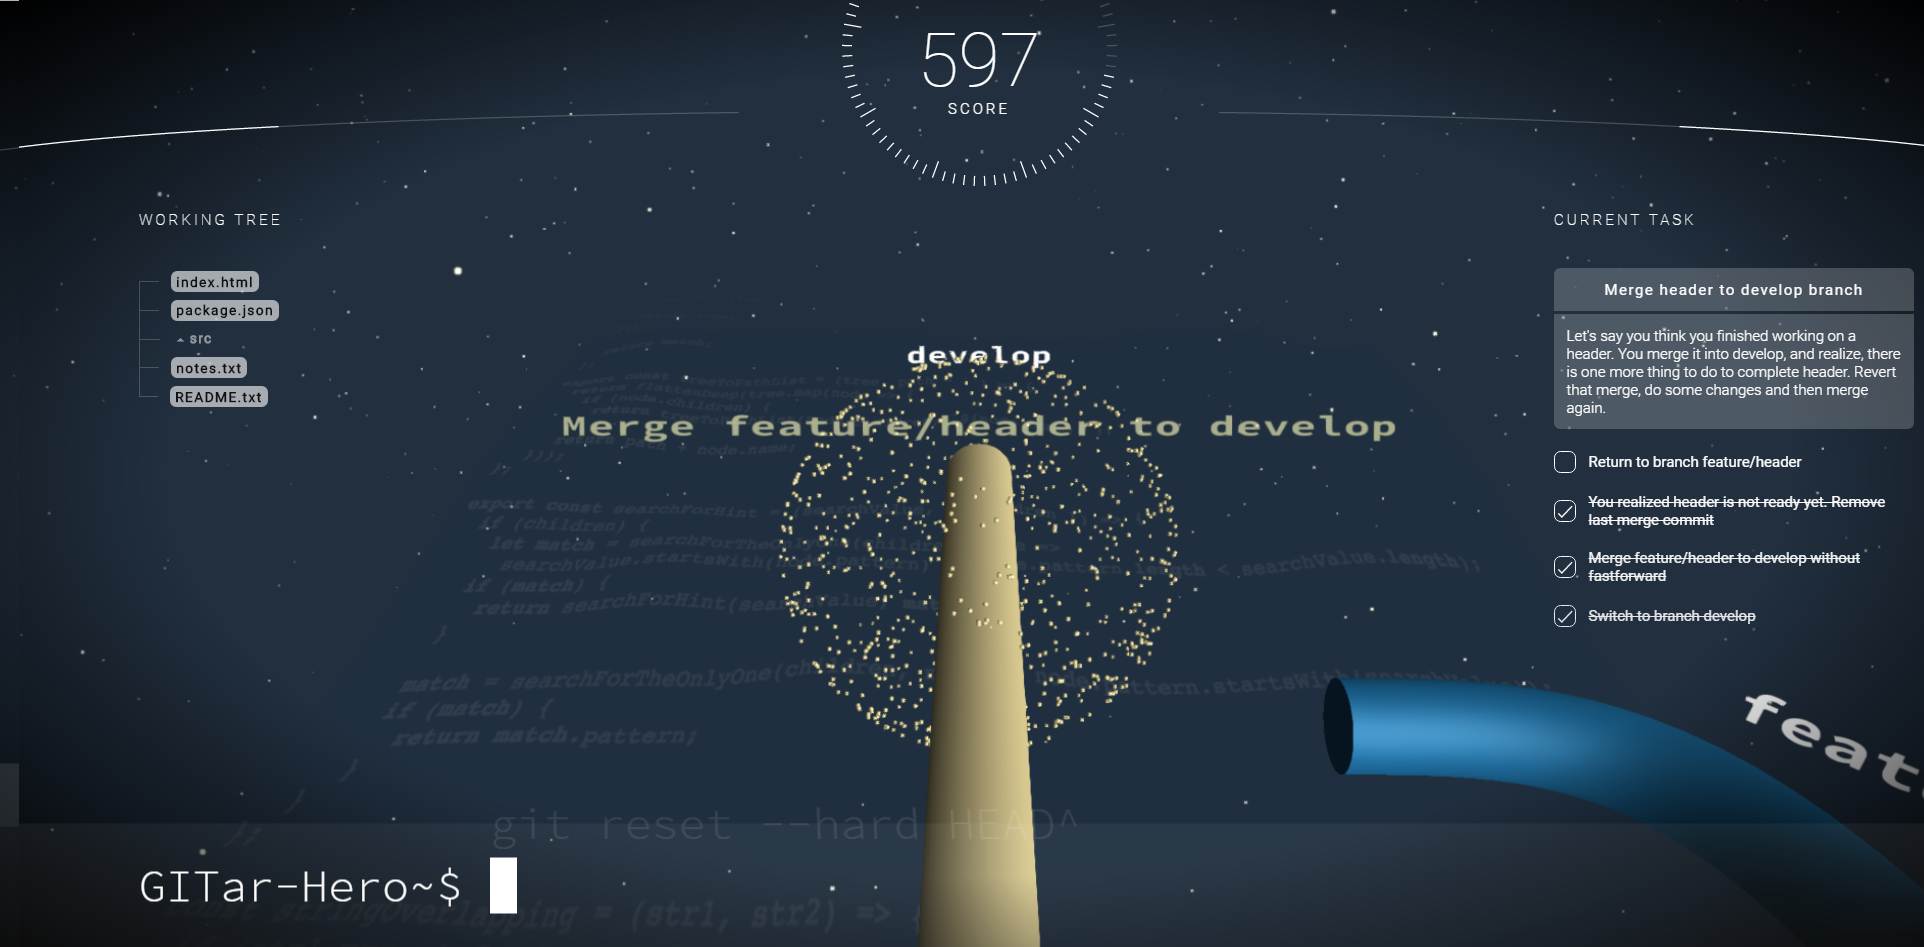
\includegraphics[width=15cm]{commit-reset}
		\caption{Animacja eksplozji rewizji}
		\label{fig:commit}
	\end{figure}

	W~kwestii wyglądu kuli zastosowane te same zabiegi co w przypadku gałęzi, na której jest umieszczona~---~posiada ten sam kolor, materiał oraz obramowanie.

	\subsection{Tekst}
	W grafice 3D niektóre obiekty, takie jak \textit{Commit} i \textit{Branch}, wymagają wyświetlania tekstu. W~przypadku obiektu rewizji jest to wiadomość i~opcjonalnie etykieta, a~dla~gałęzi nazwa.

	Tekst ukazano na płaszczyźnie dwuwymiarowej, obracającej się odpowiednio w~kierunku kamery, tak, aby niezależnie od jej położenia zawsze być do niej przodem. Ten efekt uzyskano korzystając z właściwości \textit{billboardMode} obiektu płaszczyzny dostarczanego przez bibliotekę \textit{Babylon.js}, którą ustawiono na~tryb wszystkich trzech osi układu współrzędnych.

	Dodanie tekstu do sceny wymaga wykonania kilku operacji, które zebrano w~dedykowanej do~tego celu klasie \textit{Text}. Poniżej opisano je w~odpowiedniej kolejności.

	\begin{enumerate}
		\item Utworzenie płaszczyzny o~rozmiarach wyliczonych na podstawie wielkości pojedynczego znaku. Szerokość płaszczyzny wynosi tyle, ile szerokość jednego znaku pomnożona przez liczbę liter tekstu. Ustawienie właściwości \textit{billboardMode}.

		\item Wygenerowanie tekstury z~użyciem klasy \textit{DynamicTexture} z~biblioteki \textit{Babylon.js}.

		\item Wywołanie funkcji rysującej podany tekst na teksturze, określając przy tym jego miejsce, czcionkę, kolor oraz przezroczystość tła. Kolor tekstu ustawiany jest w~zależności od obiektu nad którym ma się znaleźć, a tło jest w~pełni przezroczyste.

		\item Utworzenie materiału zawierającego zdefiniowaną wcześniej teksturę.

		\item Nadanie płaszczyźnie utworzonego materiału.
	\end{enumerate}

	Dla tekstu zdefiniowano dwie animacje~---~pojawienia się i~zniknięcia. Przy ich tworzeniu zastosowano gotowe mechanizmy z~biblioteki \textit{Babylon.js}. Aby uzyskać efekt pojawiania się stopniowo zwiększana jest wartość przezroczystości materiału płaszczyzny (od zera do jeden w ciągu jednej sekundy). Przy zanikaniu następuje mechanizm odwrotny, polegający na zmniejszaniu tej wartości od jeden do zera. Dzięki temu uzyskano efekt wygaszania.

	\subsection{Kamera} \label{camera}

	Nieodzownym elementem projektu z~grafiką~3D jest kamera. Zaimplementowano kamerę śledzącą, która rozszerza standardowe możliwości kamery \textit{FollowCamera} dostarczonej przez \textit{Babylon.js}. Najważniejszą jej zaletą jest możliwość podania obiektu, za~którym kamera będzie automatycznie podążać. Dodatkowo określa się takie parametry jak rotacja, odległość oraz wysokość z której ma spoglądać na~cel, a~także prędkość podążania i~przyspieszenie.

	\paragraph{Płynne podążanie za celem}

	Domyślnie kamera powinna być skierowana na czubek aktywnej gałęzi. W~systemie Git bieżąca gałąź przetrzymywana jest we~wskaźniku HEAD, który został omówiony w~podrozdziale~\ref{HEAD}. Może on wskazywać na gałąź lub na konkretną rewizję, a jego zmiana następuje na~skutek wykonania poleceń takich jak \textit{git~checkout}. W~repozytorium systemu Git wskaźnik HEAD jest plikiem informującym o~wskazywanym obiekcie. W~\textit{Repo3D} HEAD reprezentowany jest przez klasę \textit{HEAD}, posiadającą właściwość \textit{object3D}, w której przechowywany jest wskazywany obiekt.

	W~związku z~powyższym początkowo kamera była tak skonfigurowana, aby śledzić właściwość \textit{object3D} wskaźnika HEAD. Przemieszczała się na~skutek zmiany wskazywanego przez niego obiektu. Przełączenie aktywnej gałęzi powodowało, że~kamera samoistnie podążała nad bieżącą gałąź. Niestety w~przypadku przejścia na~znacznie oddaloną gałąź kamera zmieniała gwałtownie swoją pozycję.

	W celu zapewnienia płynnego ruchu kamery zaimplementowano dodatkową klasę \textit{CameraTarget}. Obiekt \textit{HEAD} zawiera od tego momentu dwie kluczowe właściwości~---~\textit{object3D} oraz instancję klasy \textit{CameraTarget}, który jest ustawiony jako cel kamery. W~każdej klatce porównywane są ich pozycje. Jeżeli pozycja wskazywanego przez HEAD obiektu (\textit{object3D}) różni się od~aktualnego celu kamery, to~stopniowo zmniejszana jest odległość między nimi (poprzez przesuwanie \textit{cameraTarget}). Dzięki temu nie występuje sytuacja, w której kamera byłaby gwałtownie przemieszczona do~odległego punktu. Zamiast tego płynnie podąża za~śledzonym obiektem.

	\paragraph{Podgląd całego repozytorium}

	Aby umożliwić graczowi podgląd wizualizacji całego repozytorium zaimplementowano możliwość oddalenia kamery. Podczas przewijania myszką w~tył kamera zwiększa swoją wysokość (współrzędną~Y), dopóki nie~osiągnie ustalonej wartości maksymalnej. Następnie zmniejszana jest jej pozycja wzdłuż osi~Z, do~momentu, w~którym kamera przesunie się na~początek repozytorium. Podczas przewijania w~przód następuje odwrotny proces, aż~do~powrotu kamery na~pozycję, w~której się początkowo znajdowała.

	W czasie zmiany pozycji kamery wzdłuż osi~Z w~identyczny sposób modyfikowana jest także pozycja obiektu \textit{cameraTarget}. Pozwala to~zachować stały kąt, pod jakim kamera jest skierowana wzdłuż osi~X. Ponownie wykorzystano korzyść płynącą z~rozdzielenia właściwości \textit{cameraTarget} oraz \textit{object3D}. Gdyby celem kamery był obiekt wskazywany przez HEAD (\textit{object3D}), to~nie byłoby możliwe przesunięcie go, a~w~rezultacie kąt nie byłby stały.

	\subsection{Kod w tle}

	Fabułę gry stanowi praca gracza nad repozytorium projektu informatycznego. W~celu jej uwidocznienia zdecydowano się utworzyć obiekt tła przedstawiający przewijający się kod. W pierwszej kolejności stworzono płaszczyznę przy pomocy statycznej metody \textit{CreateGround} klasy \textit{Mesh}. Aby kod nie znikał z pola widzenia, gdy kamera porusza się do przodu, w każdej klatce wartość \textit{z} wektora pozycji płaszczyzny ustawiana jest na tę samą, co wartość \textit{z}wektora pozycji kamery.

	Jako materiał wykorzystano obiekt \textit{ShaderMaterial}, który umożliwia definiowanie własnych programów cieniujących (ang. \textit{shaders}). W pierwszej kolejności dla każdego wierzchołka obiektu wykonywany jest program cieniujący przetwarzający wierzchołki (ang. \textit{vertex shader}). Jego głównym zadaniem jest odpowiednie ustawienie danego wierzchołka we współrzędnych projekcji. Dodatkowo do programu cieniującego została przekazana monochromatyczna tekstura zwaną mapą wysokości. Pozwala ona nadać płaszczyźnie wypukłości. Program cieniujący pobiera wartość kanału czerwonego z~mapy wysokości, z~miejsca określonego koordynatami tekstury (pozyskanymi w procesie \textit{mapowania UV}). Wartość ta, będąca z w przedziale od 0 do 1, jest następnie przemnażana przez stałą \textit{maxHeight} i dodawana do współrzędnej \textit{y} aktualnie przetwarzanego wierzchołka.

	\begin{figure}[h]
		\centering
		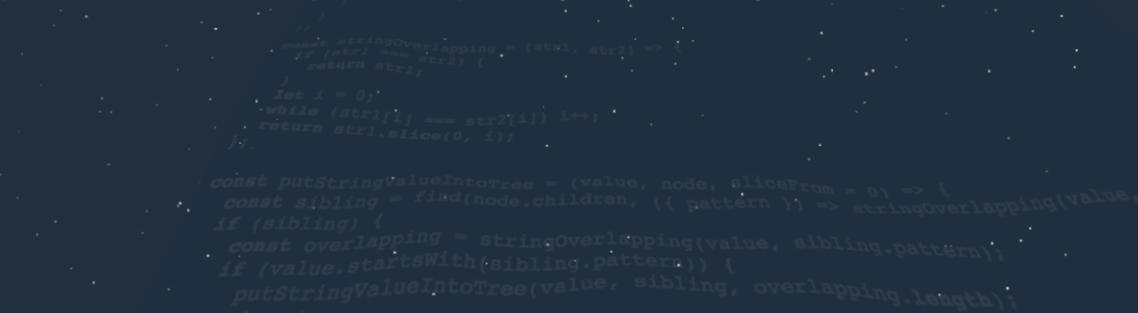
\includegraphics[width=15cm]{ground}
		\caption{Lecący w tle kod}
		\label{fig:ground}
	\end{figure}

	Zadaniem programu cieniującego przetwarzającego fragmenty (ang. \textit{fragment shader}) jest przede wszystkim naniesienie tekstury na płaszczyznę. Do programu cieniującego przekazana jest tekstura przedstawiająca biały kod na czarnym tle. Przekazane są również współrzędne tekstury, do których w każdej kolejnej klatce dodawane jest przesunięcie (w ten sposób osiągnięty został efekt przewijania tekstu). Przy użyciu tych współrzędnych, próbkowany jest kolor tekstury w odpowiednim miejscu. Jeżeli jest to kolor czarny, przetwarzany piksel pozostaje przezroczysty, w~przeciwnym wypadku kopiowany jest kolor z tekstury. W~celu podkreślenia efektu głębi obrazu zaimplementowano efekt mgły. Oznacza to, że kod znajdujący się daleko od kamery zaczyna zlewać się z tłem. Na podstawie współrzędnych fragmentu, wyliczana jest jego odległość od kamery. Ustalone zostały wartości odległości minimalnej, od której efekt mgły zaczyna być widoczny i maksymalnej, dla której fragmenty przybierają kolor tła. Dla odległości pomiędzy tymi wartościami kolor jest interpolowany liniowo między kolorem tła, a kolorem fragmentu tekstury.

	\subsection{Drobny pył}

	Poza przewijającym się kodem w~tle poruszają się także drobne cząsteczki imitujące kurz. Wypełniają one przestrzeń, niwelując wrażenie pustki.

	Do ich implementacji wykorzystany został wbudowany mechanizm \textit{ParticleSystem} biblioteki \textit{Babylon.js}. Utworzenie systemu cząsteczek wymaga podania kilku parametrów. Konieczne jest zdefiniowanie obiektu \textit{emmiter}, z którego cząsteczki będą emitowane. Innym istotnym parametrem jest tekstura, wspólna dla wszystkich cząsteczek z~danego systemu. \textit{Babylon.js} umożliwia także zdefiniowanie zakresu kierunków w~jakich będą poruszały się cząsteczki. Kolejną ważną właściwością systemu jest zakres obszaru emitującego. Domyślnie jest to środek obiektu \textit{emmiter}, ale można zdefiniować przestrzeń, w~której generowane będą cząsteczki. Dzięki temu możliwe jest skonfigurowanie systemu, z~którego cząsteczki nie są emitowane punktowo. Inne parametry jakie można ustawić to~m.in.~prędkość liniowa i~kątowa, czas, po jakim cząsteczki zanikają oraz zakres rozmiarów i~kolorów.

	Utworzono kilka obiektów emitujących cząsteczki, rozmieszczonych w~różnych miejscach sceny. Ich pozycje są określone względem celu kamery. Wraz~z~jego przesunięciem zmieniane jest także położenie \textit{emmiterów}. Dla każdego z~nich określona jest sporych rozmiarów przestrzeń w~kształcie kuli, wewnątrz której w~losowych punktach pojawiają się cząsteczki. Następnie każda z~nich powoli porusza się w~dowolnym kierunku, a~po~upływie kilku sekund delikatnie zanika.

	Zastosowanie kilku systemów cząsteczek pozwoliło~osiągnąć efekt wizualny przypominający drobinki pyłu spokojnie dryfujące w~powietrzu. Dzięki temu przestrzeń nie sprawia wrażenia pustej.

	\chapter{Podsumowanie} \label{Podsumowanie}
	
	Udało się zaimplementować grę przeglądarkową zapoznającą użytkownika z najważniejszymi poleceniami systemu Git. Opanowanie zawartych w niej materiałów powinno właściwie przygotować gracza do korzystania z programu Git, zarówno w pracy indywidualnej jak i~zespołowej. Gra GITar-Hero posiada atrakcyjny wizualnie interfejs i~dynamiczną grafikę 3D, co zapewnia bardziej zachęcającą rozgrywkę. Generowane na bieżąco kolejne zadania, jakie musi rozwiązywać użytkownik,  są dostosowane do jego umiejętności. Dzięki dostosowaniu poziomu trudności i stopniowym wprowadzaniu nowych zagadnień gracz nie zniechęca się, a nagradzanie punktami za rozwiązane polecenia dodatkowo go motywuje.
	
	Zdecydowaną zaletą stworzenia aplikacji przeglądarkowej jest jej kompatybilność oraz łatwość uruchomienia. Implementacja programu z wykorzystaniem wybranych bibliotek stworzyła wygodną warstwę abstrakcji na metody służące do interakcji z grafiką w przeglądarce internetowej. Podniosło to niezawodność aplikacji i przyspieszyło czas pracy nad oprogramowaniem.
	
	Niewątpliwą wadą przyjętego rozwiazania jest mniejsza~---~w porównaniu z aplikacjami natywnymi, opartymi na przykład o OpenGL~---~wydajność renderowania grafiki 3D przy pomocy WebGL. Spowodowało to konieczność rezygnacji z niektórych efektów graficznych, na rzecz zwiększenia płynności działania aplikacji.

	Aplikacja jest przygotowana na dalszy rozwój w wielu aspektach. Git jest rozbudowanym narzędziem; posiada wiele funkcji, które mogłyby zostać wprowadzone do scenariusza rozgrywki. Jedną z nich jest operacja zmiany bazy, której opis znalazł się w zkładce pomocy, jednak nie została ona jeszcze dodana do listy zadań. Dodatkowo, przedstawienie tej operacji za pomocą grafiki 3D stanowiłoby istotne ułatwienie w jej zrozumieniu.
	
	Systemy kontorli wersji powstały, by ułatwić współtworzenie oprogramowania przez wielu programistów w różnym czasie. Naturalnym rozwinięciem gry jest zatem wprowadzenie rozgrywki wieloosobowej. Dzięki takiemu trybowi gry, scenariusz byłby jeszcze bardziej zbliżony do realnej pracy z programem Git. Z pewnością zwiększyłoby to również zaangażowanie graczy w rozgrywkę.
	
	Istotnym aspektem gry jest konkurencja graczy. Zaimplementowany został system punktacji, jednak nie ma jeszcze centralnego rankingu graczy. Takie rozszerzenie niewątpliwie zachęciłoby większą liczbę użytkowników do rozgrywki. Stworzenie rankingu jest, z~oczywistych względów, ściśle powiązane z inną funkcją aplikacji - uwierzytelnianiem graczy. Tworzenie kont mogłoby wykorzystywać API udostępniane przez duże serwisy społecznościowe, takie jak Facebook. Kolejnym krokiem byłaby możliwość udostępniania wyniku we wspomnianych serwisach.
	
	Grywalność zależy w dużej mierze od przewidywalności zachowań aplikacji. Duże wyzwanie stanowi stworzenie rozbudowanego grafu zadań, który zapewniałby jak największą losowość w przydzielaniu zadań. Ta część aplikacji może być rozwijana w zasadzie nieustannie.

	\appendix

	\chapter{Przewodnik użytkownika}

	Praktyczne info dla opornego użytkownika, jak ma korzystać, między innymi że jest opcja scrolla aby oddalić, jakie przyciski do obsługi helpa itp. itd., krótki opis fragmentu rozgrywki co się dzieje po czym i dlaczego i jak ma na to reagować użytkownik i takie tam.

	\backmatter
	
	\begin{thebibliography}{1}
		\bibitem{progit}S. Chacon, B. Straub \emph{Pro Git} 2014, \\ https://progit2.s3.amazonaws.com/en/2016-03-22-f3531/progit-en.1084.pdf
		\bibitem{gitflow}V. Driessen \emph{A successful Git branching model} \\
		http://nvie.com/posts/a-successful-git-branching-model/
		\bibitem{gajda}W. Gajda \emph{Git. Rozproszony system kontroli wersji} Helion, 2013
		\bibitem{graphCreator} https://github.com/cjrd/directed-graph-creator
		\bibitem{babylon}http://doc.babylonjs.com/
		\bibitem{react}https://facebook.github.io/react/
		\bibitem{redux}http://redux.js.org/
		\bibitem{js}https://en.wikipedia.org/wiki/JavaScript
	\end{thebibliography}

\end{document}
